%% Copyright 1998 Pepe Kubon
%%
%% `one.tex' --- 1st chapter for thes-full.tex, thes-short-tex from
%%                the `csthesis' bundle
%%
%% You are allowed to distribute this file together with all files
%% mentioned in READ.ME.
%%
%% You are not allowed to modify its contents.
%%

%%%%%%%%%%%%%%%%%%%%%%%%%%%%%%%%%%%%%%%%%%%%%%%%%
%
%       Chapter 5
%
%%%%%%%%%%%%%%%%%%%%%%%%%%%%%%%%%%%%%%%%%%%%%%%%

\chapter[Success and Outlierness]{Success and Outlierness}
\label{chap:six}


In chapter~\ref{chap:five} we introduced the $\mid$ metric that quantifies the extent to which the individual association pattern of a potential outlier deviates from that of the whole population. The aim of this chapter is to compare the $\mid$ metric with other meaningful metrics for comparing individuals. The goal is to use the $\mid$ to estimate the value of the individuals and rank them. 
%This goal is achieved in three steps. 1) Individuals are grouped into categories. Categories can be the position of the players (e.g. defender, goalie, striker or midfielder) or the genre of the movies (action, comedy, etc.). 2) Two Bayesian network structures are learned: one from the data for the entire population, the other from individual data. 3) $\mid$  metric is computed using models learned in previous step and then used to rank the individuals.
An empirical evaluation on soccer and movie data shows a strong correlation between the $\mid$ score and success metrics: individuals that our metric identifies as unusual tend to have unusual success.

\section{Introduction}
%Predicting success especially ranking individuals has been a popular topic for statistics/machine learning research in the recent years. 

The appearance of professional soccer statistics websites has made it possible to extend statistical studies to the sports domain. One of the interesting problems in this domain is predicting success and providing true estimates of players' abilities. 
An intuitive way to estimate the value of the players is to manually aggregate information about features of individuals over time and then rank them based on their performance in those features. For example, we can compare players based on the total number of goals they have scored or the average of their shot efficiency. However, this comparison may be unfair to most players because not all players are in the position to shoot or score a goal (e.g. goalies or defenders). One may argue that defenders (or goalies) have some other characteristics that are a lot stronger in their group compared to other groups. However, detecting important and distinctive features of each group of individuals requires domain knowledge and it is not often an easy task.  \\
Another disadvantage of ranking based on manual aggregation of features is that it causes loss of information.
 
 In chapter~\ref{chap:four} and \ref{chap:five} we showed the advantage of using a generative model is to learn complex, and at the same time, informative features for individuals. 
%For instance, by using a generative model, we can find out which relation are associated and which are normally independent of each other. An advantage that can be achieved by using generative models.\\% ne  using number of matches that a player plays becomes important when the player shows high dribble efficiency and pass efficiency.  \\
In this chapter we propose a method to rank individuals which is based on $\mid$ metric introduced in chapter~\ref{chap:five}. We compare the $\mid$ metric to other metrics of success for a given domain. Our reasoning is that high success is an independent metric that indicates an unusual individual. Therefore, a correlation between log-likelihood distance and success is an independent validation of the log likelihood distance and shows that it points to meaningful and interesting outliers. 
%If the model assigns a low likelihood to generating an individual it  says something about that individual and shows how different that individuals is from normal populations. 
%A generic Bayes net (BN) structure is learned with data
%for the entire population. The nodes in the BN represent features
%for links, of multiple types, and attributes of entities,
%also of multiple types. 
%%A difference between relational and
%nonrelational data is that an individual is characterized not
%only by a list of attributes, but also by its links and by attributes
%of the individuals linked to it.
\paragraph{Approach}
Individuals are grouped into categories. A class-model Bayesian network (BN) structure is learned with data for the entire category of the individuals. An individual-model Bayesian network structured is learned  from the individual data. $\mid$ metric is computed based on the approach introduced in chapter \ref{chap:five} and is used to rank the individuals.
\paragraph{Evaluation}
We analyze two real-world data sets, from the UK Premier League and the Internet Movie Database
(IMDb). 
%The empirical distributions of the ELD metric shows that the likelihood ratios highlight individual deviations more strongly.
 Success metrics, such as the player's salary, provide an independent
score for comparison with the ELD score. The empirical distributions of the ELD metric show a strong correlation with independent success metrics.
 \section{Preliminary Analysis}
 Market value of a player is not solely based on the player's performance and is often influenced by some other factors, such as the player's age and nationality.\\
 In this section we study a few of these factors that are known to affect the market value of soccer players in the literature. We manually collected salary, nationality and age of 120 players of the Premier League in order to investigate the effect of each of these factors on the success of players.  
 \paragraph{Fact \#1: Some teams tend to pay more:} Table~\ref{table:salariofDifferentTeam} shows the average salaries of players of different teams in the Premier League. Some teams have much larger
 budgets and are able to pay higher wages compared to less wealthy teams. A player in Manchester United may not necessarily be performing substantially better than a player in the same position in Tottenham, while there is a substantial difference between the average salary of players in Tottenham and Manchester United. For this reason, we normalize the salaries of the player in order to decrease this effect. %Fortunately, after normalization, the difference between averages of salary paid by most of the teams is minor and we can expect this factor to have little effect on predicting the success.
 
%\begin{figure}
%	\centering     %%% not \center
%	{\label{fig:SalaryTeam}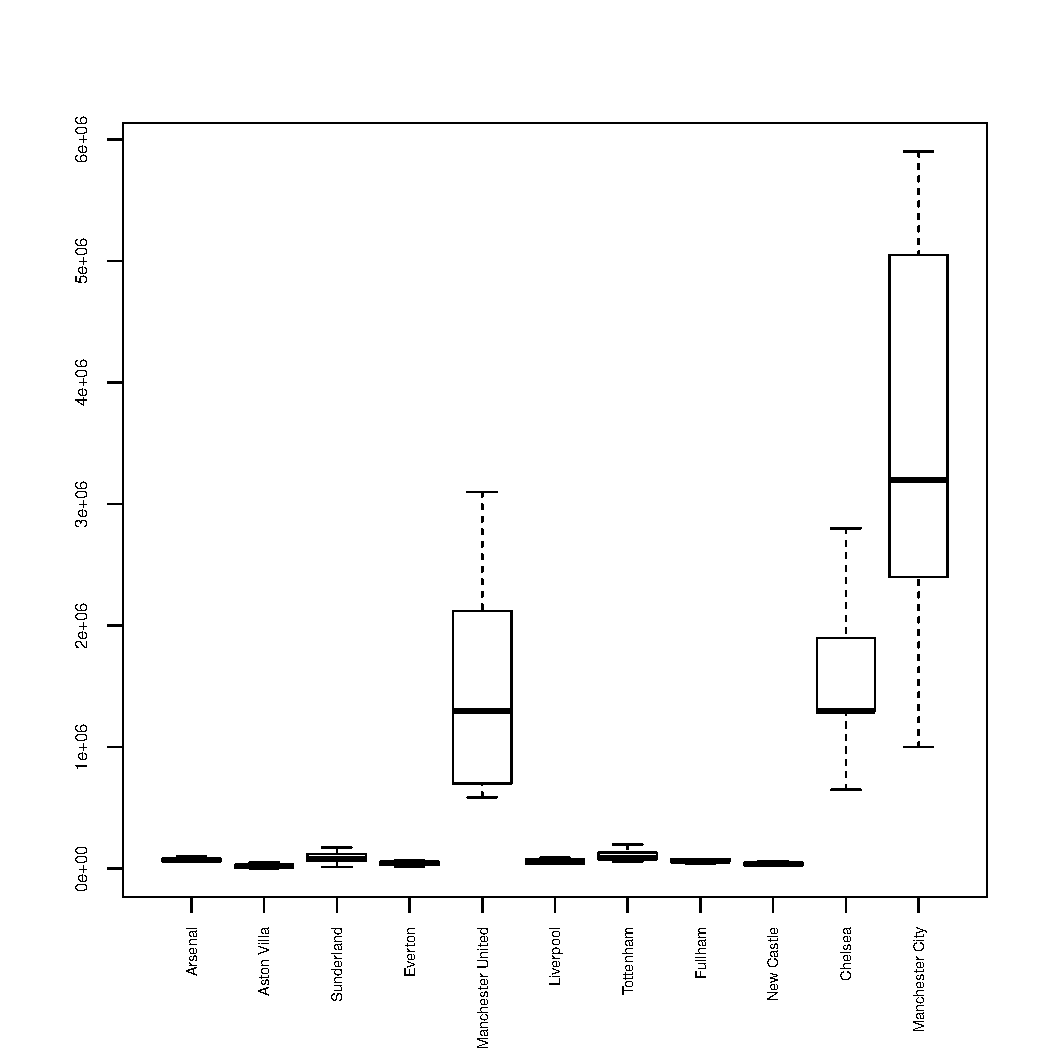
\includegraphics[width=70mm]{figures/TeamSal-2.pdf}}
%%	\subfigure[Wage bill different teams after normalization]{\label{fig:NormalizedSalary}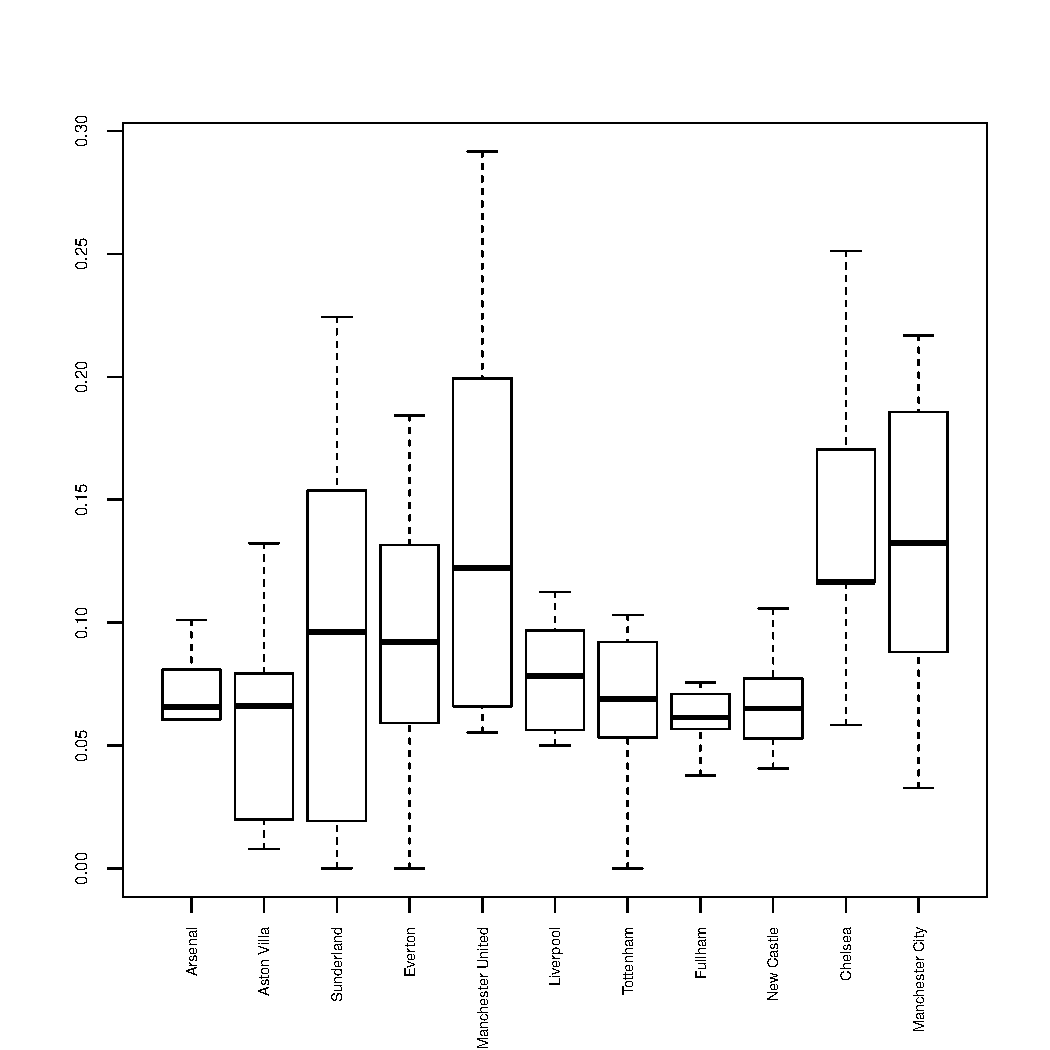
\includegraphics[width=70mm]{figures/TeamNormalSal-2.pdf}}
%	\caption{Salary of the players of different teams}
%\end{figure}



\paragraph{Fact \#2: Player's nationality has little effect on player's salary:} Previous research on soccer shows that the nationality of a player sometimes affects his salary, regardless of his performance~\cite{Wooten2013}. \\
``The phrase `Brazilian soccer player' is like the phrases `French chef' or `Tibetan monk.'  The nationality
expresses an authority, an innate vocation for the job, whatever the natural ability.''~\cite{PAPASTERGIADIS2013}\\
We investigated this phenomenon in our domain and showed that it has very little effect on the player's market value. Figure~\ref{fig:PlayersNormalizedSalary}(a) shows the distribution of salaries of the players across different nationalities.
\begin{table}[htbp]
	
	\centering
	\resizebox{0.6\textwidth}{!}{
		\begin{tabular}{|l|c|}
			\hline
			Team&$\mu$(Salary of the players of PL teams in \euro)\\\hline
			Arsenal&82307.69\\\hline
			Aston Villa&23625.00\\\hline
			Chelsea&88500.00\\\hline
			Everton&44090.91\\\hline
			Fullham&30372.57\\\hline
			Liverpool&66666.67\\\hline
			Manchester City&111076.90\\\hline
			Manchester United&81384.62\\\hline
			New Castle&41000.00\\\hline
			Sunderland&31857.14\\\hline
			Tottenham&65428.57\\\hline
		\end{tabular}}
		%
		\caption{Average salary of players in different teams .\label{table:salariofDifferentTeam}}
	\end{table}

\begin{figure}
	\centering     %%% not \center
	\subfigure[	Salaries of players of different nationalities. ]{\label{fig:SalaryTeam}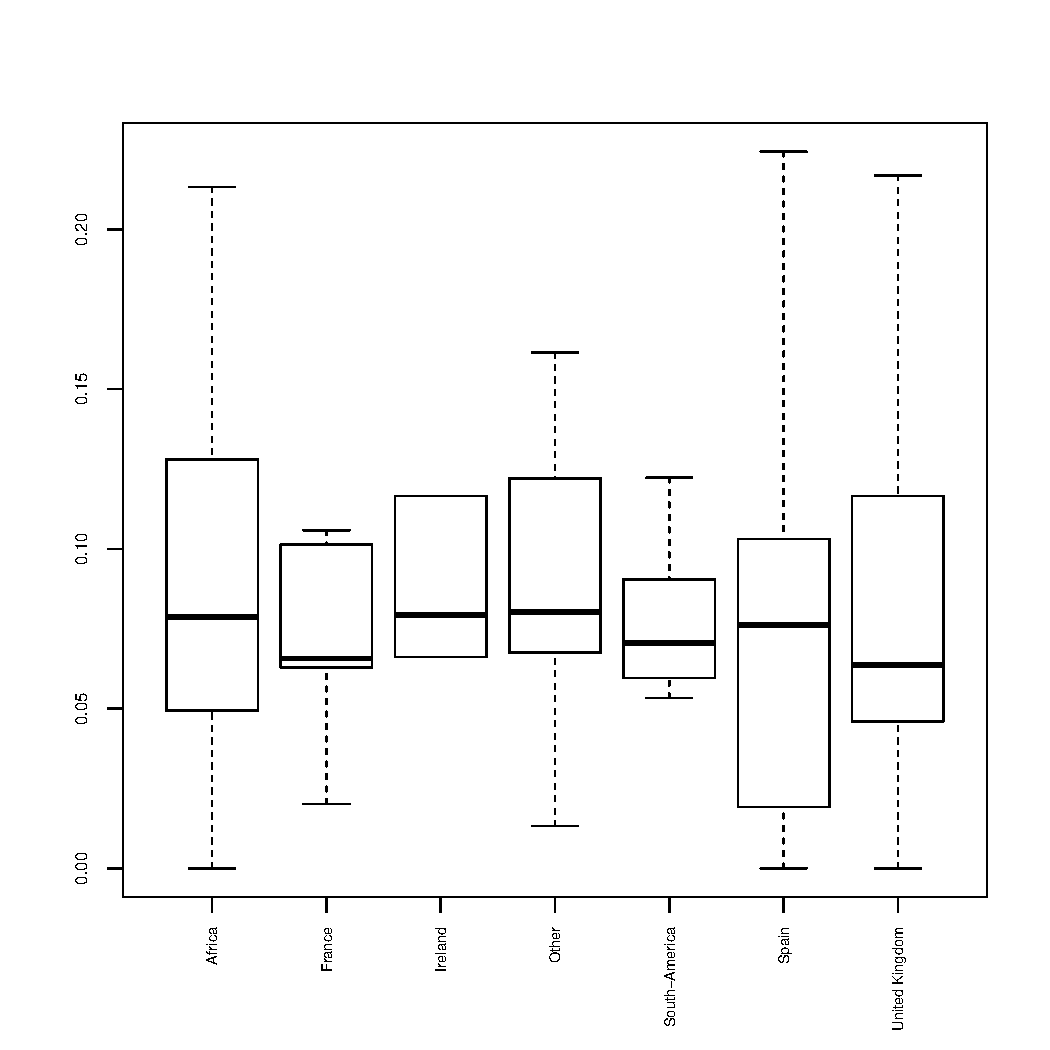
\includegraphics[width=70mm]{figures/nationalityNormalSal.pdf}}
	\subfigure[	Salaries of players of different age group. ]{\label{fig:b}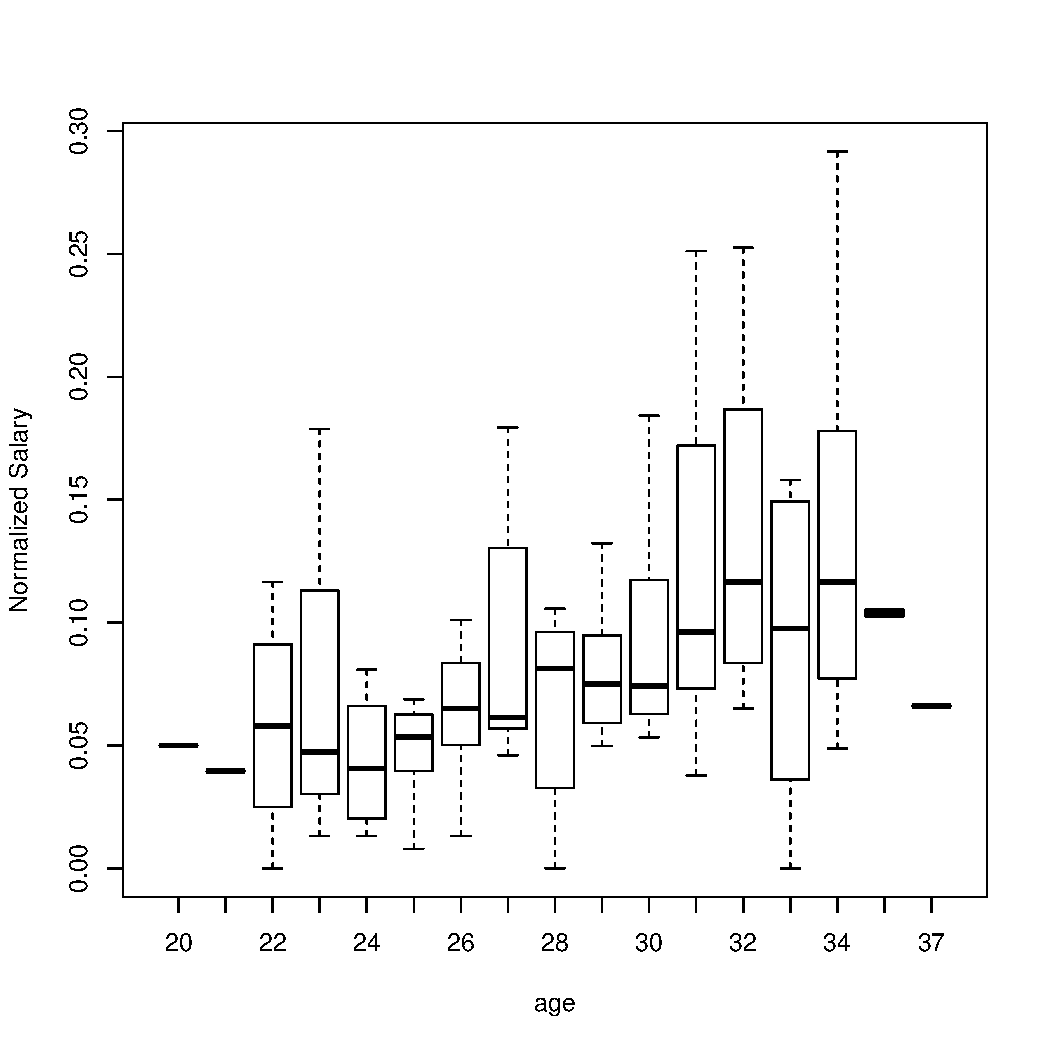
\includegraphics[width=70mm]{figures/PlayersNormalizedSalary.pdf}}
	\caption{Salary comparison of Premier League Players}\label{fig:PlayersNormalizedSalary}
\end{figure}

%\begin{figure}[t]
%	\centering
%	\includegraphics[width=0.6\textwidth] 
%	{figures/nationalityNormalSal.pdf}
%	\caption{
%		Salaries of players across different nationalities. 
%		\label{fig:nationalitySalary}
%	}
%\end{figure}

\paragraph{Fact \#3: Player's salary increases as age increases:}
Older players, from ages 30 to 33, tend to earn higher wages compared to other age groups because it takes time to accumulate fame and experience. A famous older player and a young player may play equally well, but the famous player may have a higher salary due to his reputation. \\
For each player salary distribution has a different peak, but it is between 30-33 for most players~\cite{schwartz}. Figure~\ref{MetricComputation} shows the salary of the players in different age groups.

Based on the points discussed above, we know that a method that is solely based on players' performance will not be 100\% successful in ranking the players. 
% Please note this fact is not in favour of our method too.

%\begin{figure}[t]
%	\centering
%	\includegraphics[width=0.6\textwidth] 
%	{figures/PlayersNormalizedSalary.pdf}
%	\caption{
%		Salaries of players in different age. 
%		\label{fig:nationalitySalary}
%	}
%\end{figure}
%\begin{figure}[t]
%	\centering
%	\includegraphics[width=0.7\textwidth] 
%	{figures/TeamSal.pdf}
%	\caption{
%		%We show only the Markov blanket of the Results node to simplify. 
%		\label{fig:bns}
%	}
%\end{figure}
%\begin{figure}[t]
%	\centering
%	\includegraphics[width=0.7\textwidth] 
%	{figures/TeamSal.pdf}
%	\caption{
%		%We show only the Markov blanket of the Results node to simplify. 
%		\label{fig:bns}
%	}
%\end{figure}

\section{Related Work }
%Performance assessment is an important tool for operational analysts in many areas. For example, performance of traders or engineers is assessed by fund managers\cite{Grinblatt1989,Swamidass1987}.\\
\subsection{Analyzing sports data}
 Analyzing sports data can make a significant difference in scoring players, signing contracts and preventing injuries. Pei{~\em et al.}\cite{Pei2006} propose a reference-based method that uses relative degree of density with respect to a fixed set of reference points to calculate the neighbourhood density of a data point. They aim to find outstanding players based on two test settings: 1) The total number of games played, goals scored and shooting percentages. 2) Points scored, plus/minus statistics and penalty minus. \\
Schwartz~\cite{schwartz} {~\em et al.} focused on the valuation of draft order in the SuperDraft. The valuation of draft order was first introduced in the National Football League and proved very useful to the coach in trading players. They first estimate career trajectories of players and then assess the value of the draft position by introducing some performance measure. They used time played and salary of the player as ground truth in order to validate their method.

 
\subsection{Ranking system in Sports domain}
Ranking individuals is a useful task for many applications in Information Retrieval, Natural Language Processing and Data mining.
 In sports, performance is usually interpreted as a rating system or ranking system. Ranking players is particularly important in this domain because teams with lower budgets are usually looking for ways to detect undervalued players to be able to compete with wealthier teams for lower costs.
Lewis {\em et. al}~\cite{Lewis2003} used a quantitative analysis to evaluate the value of baseball players. \\
In the individual sports (e.g. tennis), ranking is straightforward and can be driven from the results of past tournaments, as it has been done  for years by the Association of Tennis Professionals (ATP). However, this simple framework for ranking has been questioned and claimed to perform poorly in predicting the results of future games~\cite{McHale2011}. Other sports associations, such as soccer and cricket, also have official rankings of teams and players, which is the basis of many important decisions. For example, FIFA's world ranking plays an important part in awarding work permits to players outside the European Union in the Premier League~\cite{McHale2012}.
 The problem of ranking teams and players is not trivial and the need for a better analytical system should not be understated. Although the world ranking performs poorly in predicting match outcomes, it has been used to determine qualifications for tournaments~\cite{McHale2007}.
 
 In team sports, rating individuals is a more complex task due to team structure; players have different positions. Keri {\em et. al} have developed a rating system for each speciality in baseball~\cite{Keri2006}.
 
 The analysis becomes more complicated when the goal is to compare players with different specialities. Goldman {\em et al.} investigates the metrics that attempt such an analysis in baseball and value players regardless of their position~\cite{Goldman2010}.
 % Lewis 2005 has explored methodologies for such rating system for Cricket. 
  McHale{~\em et. al} developed an index to rate players regardless of their playing speciality, based on their contributions to wining performances~\cite{McHale2012}. 
 


%\section{Experiments}
%We show the distribution of the ELD values on the Soccer and the IMDb datasets.
%
%\subsection{Datasets}
%Similar to the other chapters, data tables are prepared from Opta data~\cite{opta-original} and IMDb~\cite{IMDB-original}. Table~\ref{table:Features} lists the populations and features. Table~\ref{table:Stats} shows summary statistics for the datasets. 
%\begin{table}
%	\centering
%	\resizebox{0.7\textwidth}{!}{
%		\begin{tabular}{|l|l|l|l|} \hline
%			\multicolumn{2}{|c|}{Premier League Statistics}& \multicolumn{2}{|c|}{IMDB Statistics}\\
%			\hline
%			Number Teams&20&Number Movies&3060 \\ \hline
%			Number Players&484&Number Directors&220 \\ \hline
%			Number Matches&380&Number Actors&98690  \\ \hline
%			avg player per match&26.01& avg actor per movie&36.42  \\ \hline
%		\end{tabular} 
%	}
%	\caption{Summary Statistics for the IMDB and Soccer data sets}
%	\label{table:Stats}
%\end{table}
%
%
%\begin{table}[htbp]
%	\centering
%	\resizebox{0.6\textwidth}{!}{
%		\begin{tabular}{|c|p{5cm}|}
%			\hline
%			Individuals & Features\\ \hline
%			\begin{tabular}{c}Soccer-Player\\per Match \end{tabular} & $\it{TimePlayed}$,$\it{Goals}$,$\it{SavesMade}$,
%			$\it{ShotEff}$,$\it{PassEff}$,$\it{WinningGoal}$,
%			$\it{FirstGoal}$,$\it{PositionID}$, $\it{TackleEff}$,$\it{DribbleEff}$,
%			$\it{ShotsOnTarget}$ \\ \hline
%			\begin{tabular}{c}Soccer-Team\\per Match \end{tabular} & $\it{Result}$,$\it{TeamFormation}$,
%			$\sum\it{Goals}$,$\mu\it{ShotEff}$,$\mu\it{PassEff}$,
%			$\mu\it{TackleEff}$,$\mu\it{DribbleEff}$. \\ \hline
%			IMDB-Actor & $\it{Quality}$, $\it{Gender}$ \\ \hline
%			IMDB-Director & $\it{Quality}$,$\it{avgRevenue}$\\ \hline
%			IMDB-Movie&$\it{year}$,$\it{isEnglish}$,$\it{Genre}$,$\it{Country}$, $\it{RunningTime}$, $\it{Rating}$ by User\\ \hline
%			IMDB-User& %$\it{Rating}$,
%			$\it{Gender}$, $\it{Occupation}$.\\ \hline
%		\end{tabular}}
%		\caption{Attribute Features.% $\mu$ = average, $\\sum$ = sum. For relationships please see text.
%			\label{table:Features}}
%		
%	\end{table}
\section{Correlation with Success}
\label{sec:success}

%OS: I put previous writing after \end{document}
%\subsection{Experiments}
%\subsubsection{Datasets}

The aim of this section is to compare the $\mid$ metric with other meaningful metrics for comparing individuals. Our reference metrics are success rankings of individuals selected for a specific domain, shown in table~\ref{table:metrics}. We use the same data as in our other experiments, as described in chapter~\ref{chap:three}. 

Success rankings are one of the most interesting features to users. Strong correlations between the $\mid$ metric and meaningful success metrics provide evidence that the $\mid$ metric is also meaningful. We measure correlation strength by the standard correlation coefficient $\rho$. The coefficient ranges from -1 to 1, where 0 means no correlation and 1 or -1 indicates maximum strength~\cite{Fisher1921}.

The observed correlations are remarkable in at least two respects: 1) The strength of the correlation between the $\mid$ metric and the success ranking are high; coefficients range from 0.45 to 0.82. 2) We observe this phenomenon across different domains, different types of individuals and different success metrics.


\begin{table}[htbp]
	
	\centering
	\resizebox{0.8\textwidth}{!}{
		\begin{tabular}{|l|l|l|l|l|l|}
			\hline
			Dataset&Success Metric&Min&Max&Standard Dev.&Mean\\ \hline
			IMDb & Sum of Rating & 1 & 14795 & 1600.22 & 1057.58\\ \hline
			Soccer-Player &TimePlayed& 5.0 & 3420 & 1015.69 & 1484.0\\ \hline
			Soccer-Player&Normalized Salary&0.007&0.28&0.620&0.100\\\hline
			Soccer-Player&Sum of Shot Efficiency&0&82&9.87&6.53\\\hline
			Soccer-Team &Standing& 1.0 & 20 & 5.91 & 10.5\\ \hline
			
		\end{tabular}}
		\caption{Success metrics and their distributions.\label{table:metrics}}	
	\end{table}
	
	
	
	For a population with a diverse set of skills and resources,
	%apart from a serious decline in quality of generalization, 
	being different from the generic class can be interpreted as both exceptionally better or worse than normal population. In the domains we study in this data, we found that higher $\mid$ scores indicate exceptionally good individuals. Our interpretation of this positive correlation between $\mid$ and success is that our domains featured skilled individuals, such that the average is already quite successful. 
	For example, in the Premier League we expect most players to be in the range of good players. Therefore, deviating from the rest of the population is a signal for detecting exceptionally good players. Our $\mid$-success scatterplots below provide empirical evidence for this interpretation; we typically see a large cluster of individuals around the origin, meaning that their success is normal and their $\mid$ score is low.
	
	\subsection{Methodology}
	
	We report the correlations between the $\mid$ metric and metrics of success for a specific domain. We also focus on some unusually successful individuals as case studies. 
	In considering the correlation between $\mid$ and success, it is useful to investigate subgroups of individuals to ensure an apples-to-apples comparison~\cite{Sun2009}. For instance, the attributes that lead to success are different for strikers and goalies.  Accordingly, we report correlations for subgroups as well as entire classes of individuals. 
	
	%	Another point to consider is that, in BN generalization, similar to statistical generalization, population size and the structure of the  individuals is important. For example, in the Premier League, when the goal is to predict the success of  teams, there is no strong correlation between the ELD metric and standing of the teams as we expected it to be similar to the other domain/individuals ($\rho(Standing, ELD)=-0.21$). This could be due to the diverse and yet very small population (20 teams in total). But when we decrease diversity by evaluation only top 10 teams in the Premier League standing, correlation becomes a lot more stronger ($\rho(Standing, ELD)=-0.71$).
	
	
	\subsection{Correlations between the $\mid$ outlier metric and success}
	
	The next three tables summarize the observed correlations between success and $\mid$ metrics: Teams in Table~\ref{table:teamELD}, Players in Table~\ref{table:ELDwithPlayer},  Movies in Table~\ref{table:ELDmovie}.

		
		
		
		%\begin{table}[htbp]
		%	\caption{Correlation between $\mid$ metric and success metric of Goalies . \textbf{make single table. Probably make the rows the metrics, the columns the classes, including the whole population. Or add a row for all players. See our aaa2014.tex paper. } \label{table:players}}
		%	\centering
		%	\resizebox{0.7\textwidth}{!}{
		%		\begin{tabular}{|c|c|c|c|}
		%			\hline
		%			Metric&Sum of SavesMade&TimePlayed&Salary\\\hline
		%			$\mid$&0.71&0.73&0.6\\\hline
		%		\end{tabular}}
		%		\caption{Correlation between $\mid$ metric and success metric of Midfielders. \label{table:Midfielders}}
		%		\resizebox{1\textwidth}{!}{
		%			\begin{tabular}{|c|c|c|c|c|}
		%				\hline
		%		Metric&Sum of Pass Efficiency&Sum of dribble Efficiency&TimePlayed&Salary\\\hline
		%		$\mid$&0.89&0.76&0.80&0.45\\\hline
		%			\end{tabular}
		%			
		%			}
		%				\caption{Correlation between $\mid$ metric and success metric of Strikers .\label{table:strikers}}
		%					\resizebox{0.7\textwidth}{!}{
		%						\begin{tabular}{|c|c|c|c|}
		%							\hline
		%							Metric&Shots On Target&TimePlayed& Salary\\\hline
		%							$\mid$&0.72&0.82&0.79\\\hline
		%						\end{tabular}
		%						
		%					}
		%\caption{Correlation between $\mid$ metric and success metric of Movies .\label{table:movie}}
		%\resizebox{0.8\textwidth}{!}{
		%	\begin{tabular}{|c|c|c|c|}
		%		\hline
		%	Genre&Sum of Rating&Average of Rating&Number of Rating\\\hline
		%	Action&0.68&0.30&0.72\\\hline
		%	Drama&0.78&0.29&0.81\\\hline
		%	Comedy&0.85&0.41&0.84\\\hline
		%	All Movies&0.56&0.17&0.60\\\hline
		%		\end{tabular}
		%}
		%		\end{table}
		%		
		%
		
		\begin{table}
			\caption{Correlation between $\mid$ metric and success metric of Movies.\label{table:ELDmovie}}
			\centering
			\resizebox{0.8\textwidth}{!}{
				\begin{tabular}{|c|c|c|c|}
					\hline
					Genre&Sum of Rating&Average of Rating&Number of Rating\\\hline
					Action&0.68&0.30&0.72\\\hline
					Drama&0.76&0.32&0.77\\\hline
					Comedy&0.85&0.41&0.84\\\hline
					All Movies&0.56&0.17&0.60\\\hline
				\end{tabular}
			}
		\end{table}
		
		
			
			\begin{table}
				\caption{Correlation between $\mid$ metric and standing of Teams. The best standing is place 1. \label{table:teamELD}}
				\centering
				\resizebox{0.4\textwidth}{!}{
					\begin{tabular}{|c|c|}
						\hline
						Team&Standing\\\hline
						Top Teams&-0.71\\\hline
						Bottom Team&-0.33\\\hline
						All Team&-0.20\\\hline
					\end{tabular}
				}
			\end{table}
			
			
			\begin{table}
				\caption{Correlation between $\mid$ metric and success metrics of Players.}
				\label{table:ELDwithPlayer}
				\centering
				\resizebox{1\textwidth}{!}{
					\begin{tabular}{|c|c|c|c|c|c|}
						\hline
						Class&TimePlayed&Salary&SavesMade&ShotsOntarget&Passeff\\\hline
						Strikers&0.76&0.79&NA&0.72&NA\\\hline
						Midfielders&0.73&0.45&NA&NA&0.89\\\hline
						Goalies&0.69&NA&0.71&NA&NA\\\hline
						All players&0.81&0.56&NA&NA&NA\\\hline
						%Synthetic&40&280\\ \hline
					\end{tabular}}
					
				\end{table}
		
		
		\subsubsection{Teams} 
		\paragraph{Team Standing}
		The most successful team has Standing=1 and the least successful team has Standing=20 in the 2011-2012 Season. For the top teams, a very strong negative correlation emerges between $\mid$ and standing: teams with higher $\mid$ achieve a better (lower) standing. 
		
		Figure~\ref{fig:TeamStandingELD} shows the correlation of $\mid$ with team success metrics in a scatter plot. The top two teams, Manchester City and Manchester United, stand out strongly in terms of the $\mid$ metric (bottom right corner).
		
		\begin{figure}[t]
			\centering
			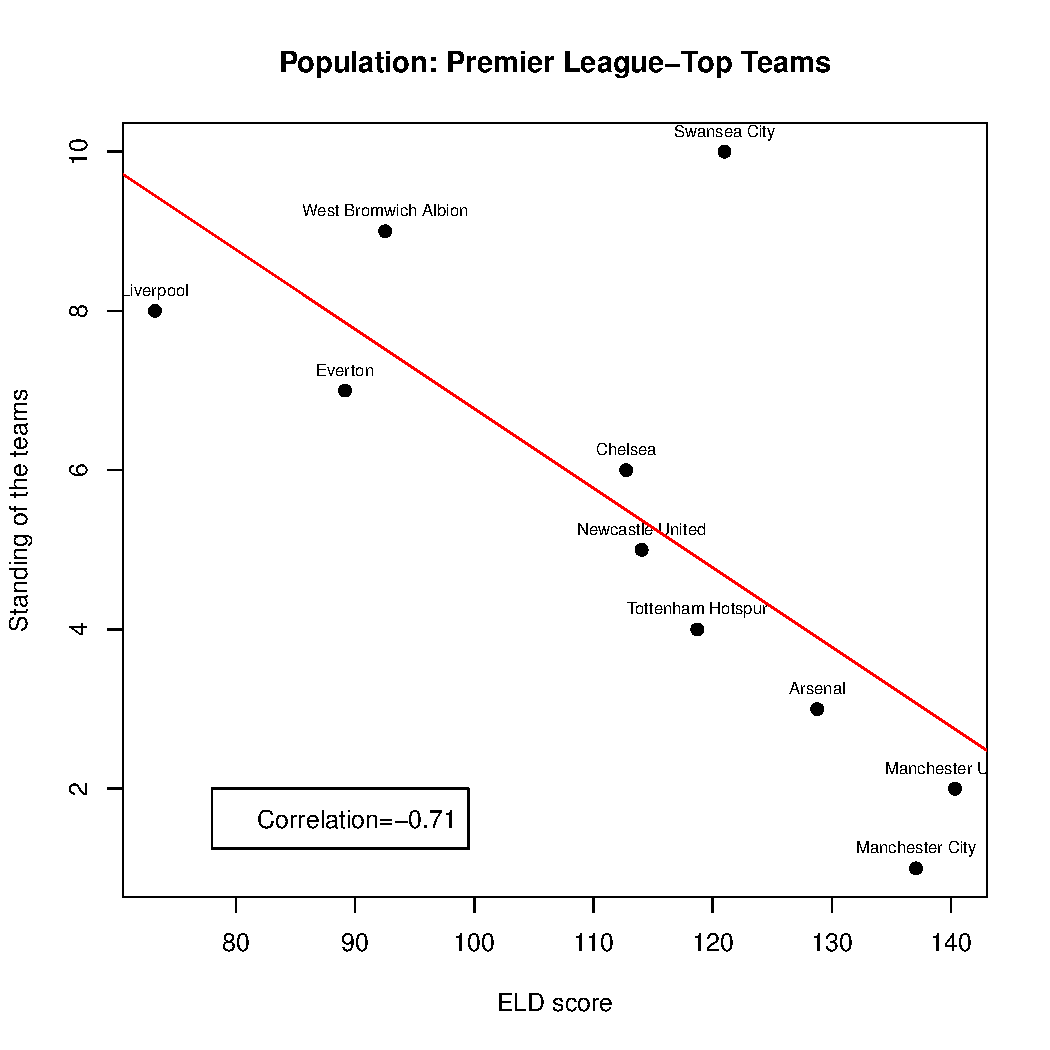
\includegraphics[width=0.5\textwidth]{NewPlotsJan2016/topTeamStats-Sep.pdf}
			
			\caption{Teams: Team Standing vs. $\mid$ for the top teams in the Premier League. 
				\label{fig:TeamStandingELD}}
		\end{figure}
		
		\subsubsection{Players}
		
		\paragraph{Players Time Played} is the total time that a player played over all matches in the season. This metric was shown to correlate strongly with other success metrics, such as salary, on MLS soccer data~\cite{schwartz}. 
		%	Tables ~\ref{table:goalie} and \ref{table:players} 
		%	
		%	and Figures \ref{fig:GoalieTime} and \ref{fig:StrikerTime} 
		%	
		%	show the correlation between the ELD metric and time played. 
		For each subgroup there is a strong positive correlation with $\mid$, meaning that atypical players with higher $\mid$ tend to play more minutes.
		
		%The results are mixed; they show that pay cannot be adequately explained by past performance
		%	alone, nor are pay levels justified by future performance. The bids for players in the initial
		%	auction appear to have been based on intangibles that are hard to quantify%
		\paragraph{Salary} is probably the most obvious, and at the same time often the most misleading way to measure success of the players. Previous studies suggest that salary of the players does not  always follow their performance in many sports, such as baseball and soccer~\cite{Hall2002,Barrio2004}. They show that pay cannot be explained only by past performance and there are other factors that are hard to quantify and have a great effect on the salaries. 
		
		We manually collected the salaries of 120 players that we could find on-line. Table \ref{table:ELDwithPlayer}  and Figures~\ref{fig:strikersELD} and \ref{fig:goaliesELD} show the correlation between $\mid$ and this success metric. The correlation is high, especially for Strikers. We discuss the relatively weaker salary correlation for midfielders in more detail below.
		
		\paragraph{Shots on Target} applies to strikers only. This is defined as any shot attempt that would, or does, enter the goal if left unblocked. We record the total number of these shots over all matches of the strikers only. This metric was shown to correlate strongly with $\mid$ (see Table \ref{table:ELDwithPlayer}, Figure~\ref{fig:StrikerShot}).
		
		Figure~\ref{fig:strikersELD} plots $\mid$ against striker success metrics. We observe a large cluster around the origin, which points to a large base of normal strikers with both salaries and low $\mid$ scores. %The striker with the greatest $\mid$ score is Robin van Persie; he stands out in terms of Shots on Target, Time Played, and Salary. 
		
		%should probably label the points with individual names
		
		
		\begin{figure}
			\centering     %%% not \center
			\subfigure[Strikers: Salary vs $\mid$. ]{\label{fig:StrikerSalary}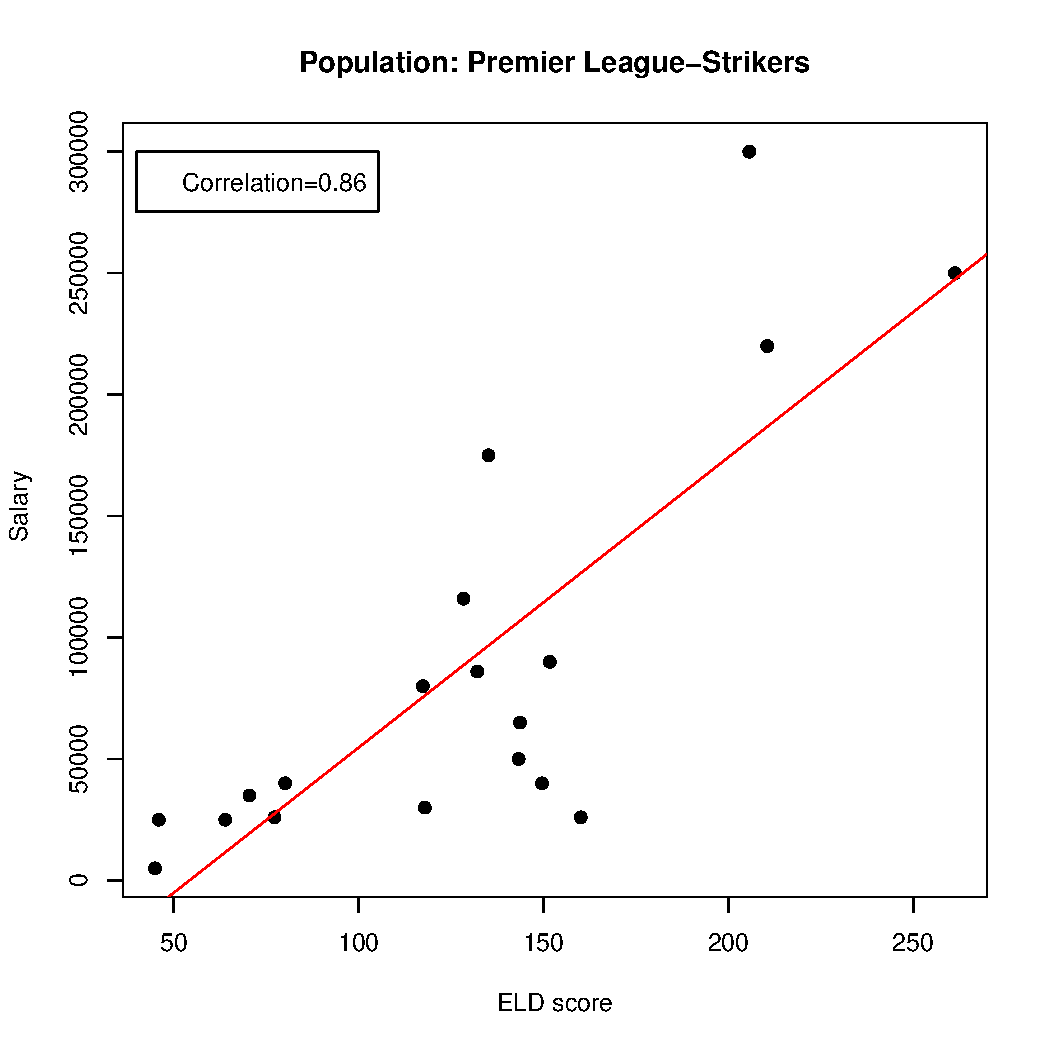
\includegraphics[width=0.48\textwidth]{NewPlotsJan2016/1d-sumStrikerSalary.pdf}}
			\subfigure[Strikers: Shots On Target vs $\mid$]{\label{fig:StrikerShot}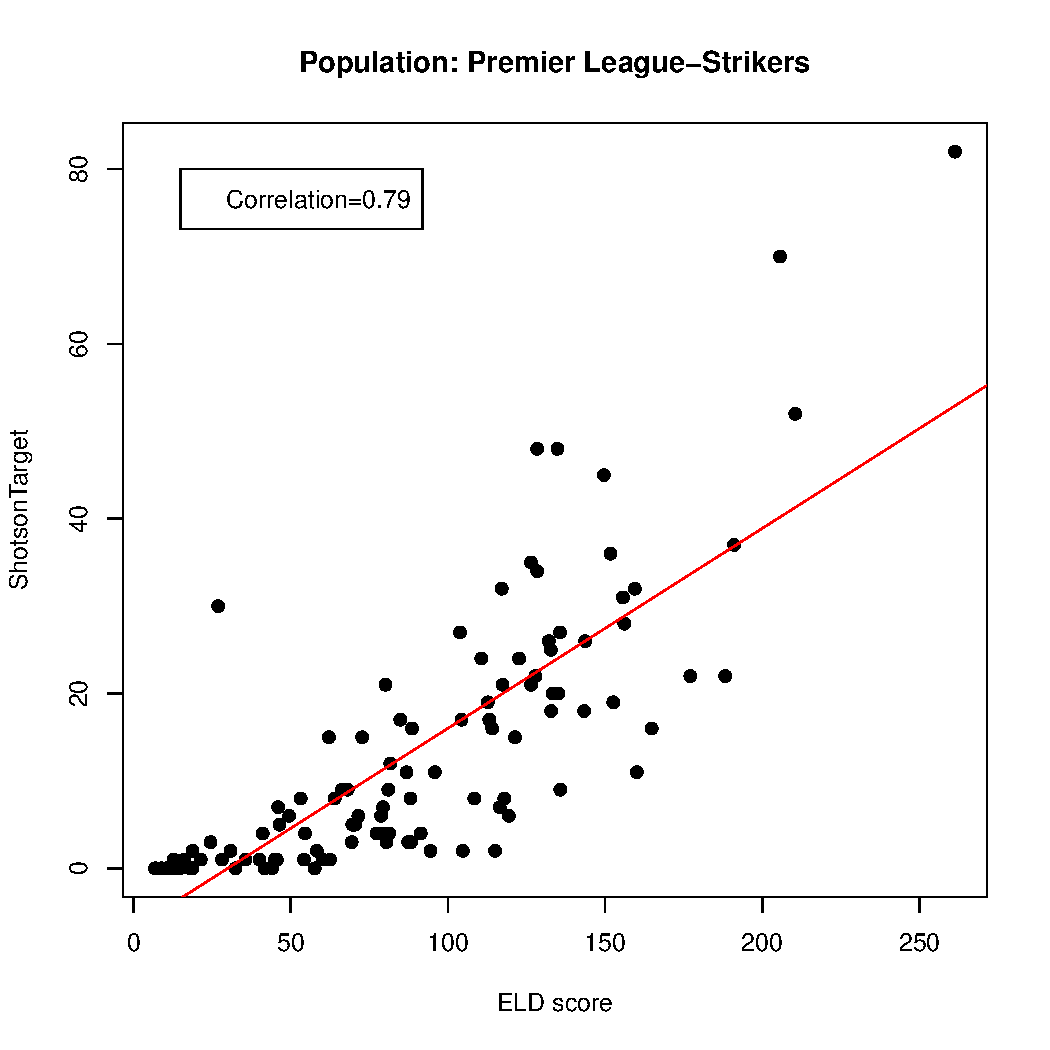
\includegraphics[width=0.5\textwidth]{NewPlotsJan2016/1d-ShotsonTarget-sumStrikerStatistics.pdf}}
			\subfigure[Strikers: Time played vs $\mid$.]{\label{fig:StrikerTime}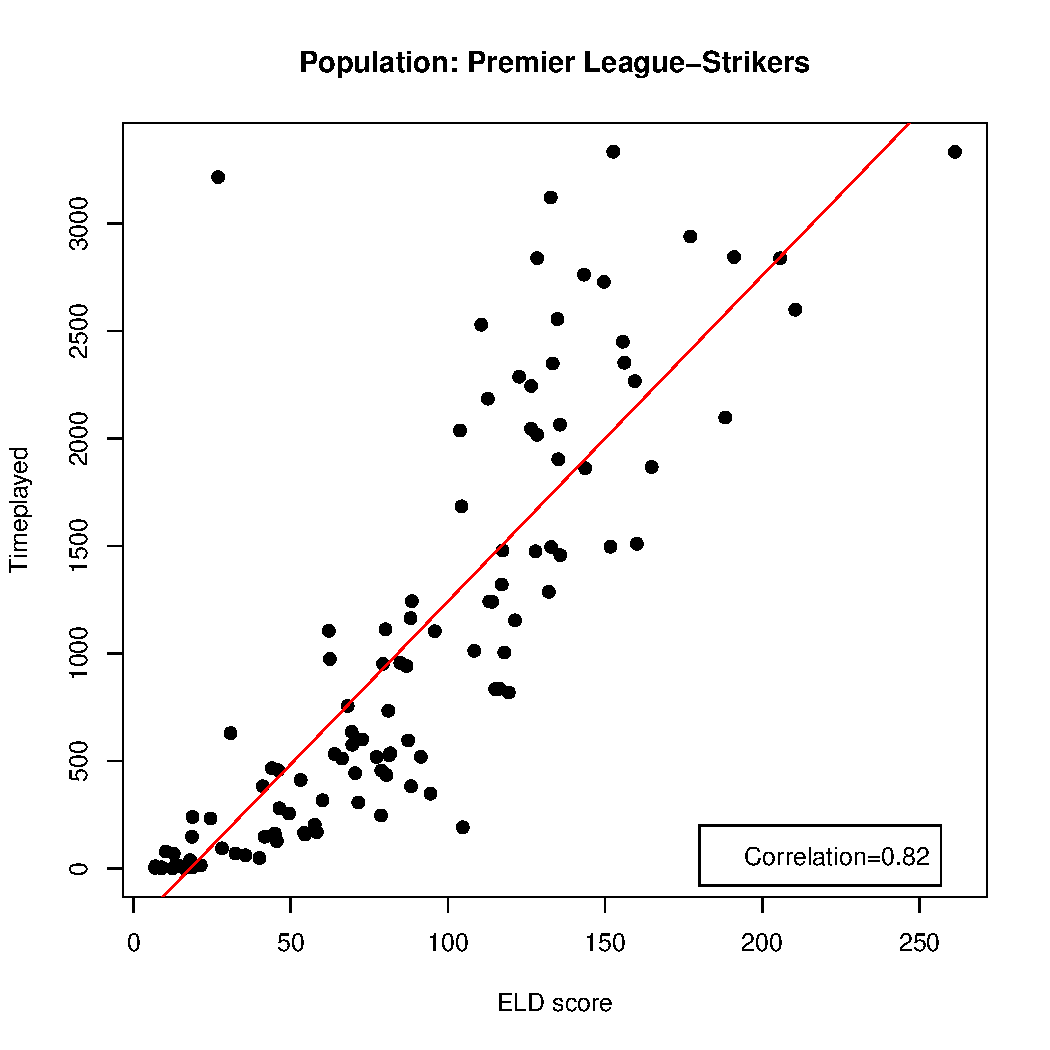
\includegraphics[width=0.5\textwidth]{NewPlotsJan2016/1d-sumStrikerStatistics.pdf}}
			\caption{Correlations in the strikers population\label{fig:strikersELD}}
		\end{figure}
		
		
		
		\paragraph{Saves Made} applies to goalies only; it is defined as the total number of saves that goalies made over all the matches. This metric shows a strong correlation with $\mid$ as well (see Table~\ref{table:ELDwithPlayer}, Figure~\ref{fig:GoalieSaves}).  
		
		Figure~\ref{fig:goaliesELD} shows the correlation of $\mid$ with goalie success metrics in a scatter plot. Goalies do not vary much in terms of the time they play. Wayne Hennessey has the highest number of Saves Made and also an unusually high $\mid$ score, although not the highest. 
		
		
		
		\begin{figure}
			\centering     %%% not \center
			\subfigure[Goalies: sum of time played vs $\mid$. ]{\label{fig:GoalieTime}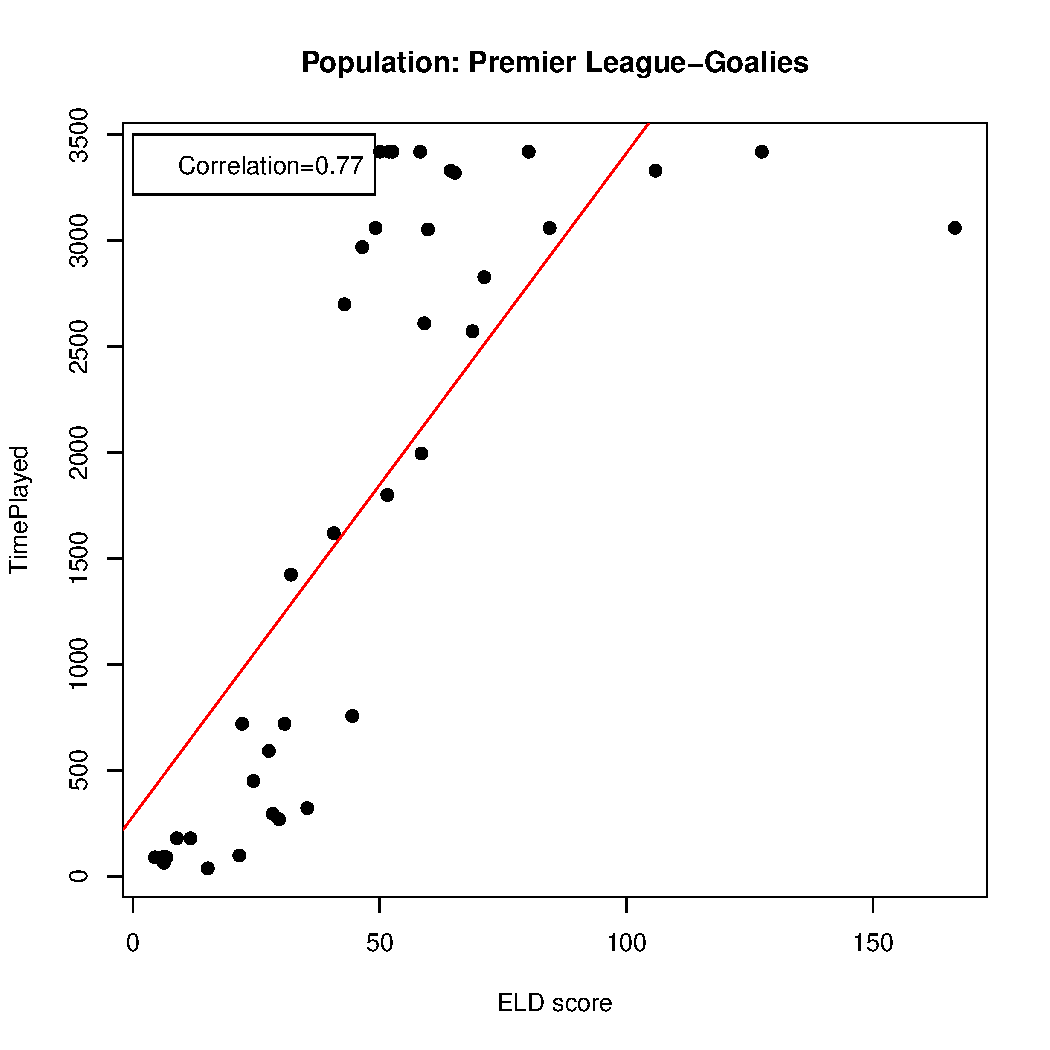
\includegraphics[width=0.48\textwidth]{NewPlotsJan2016/sumGoalieStatistics.pdf}}
			\subfigure[Goalies: sum of saves made vs $\mid$]{\label{fig:GoalieSaves}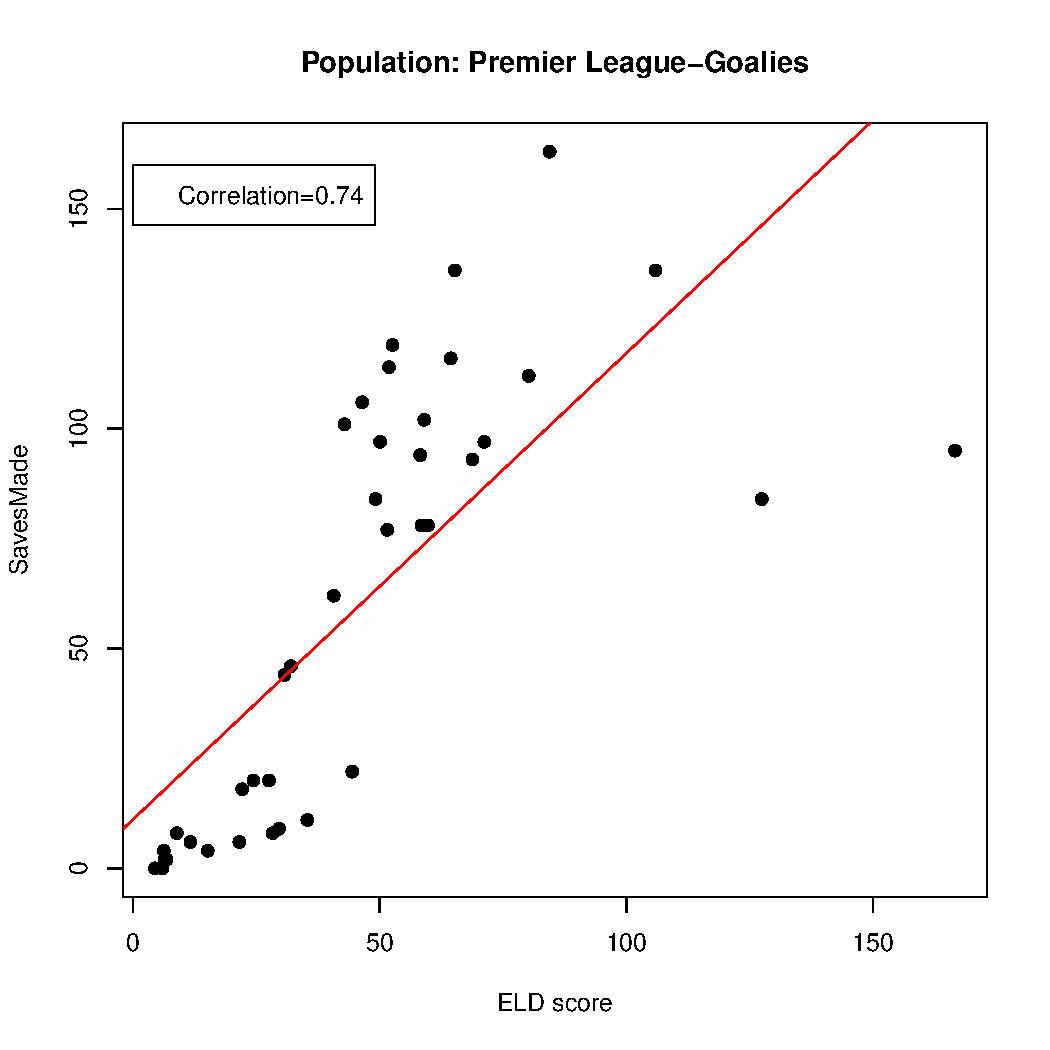
\includegraphics[width=0.5\textwidth]{NewPlotsJan2016/sumGoalieStatisticsSavesMade.pdf}}
			%	\subfigure[Teams: Team Standing vs. $\mid$ for the top teams in Premier League. \textbf{separate figure please}]{\label{fig:TeamStanding}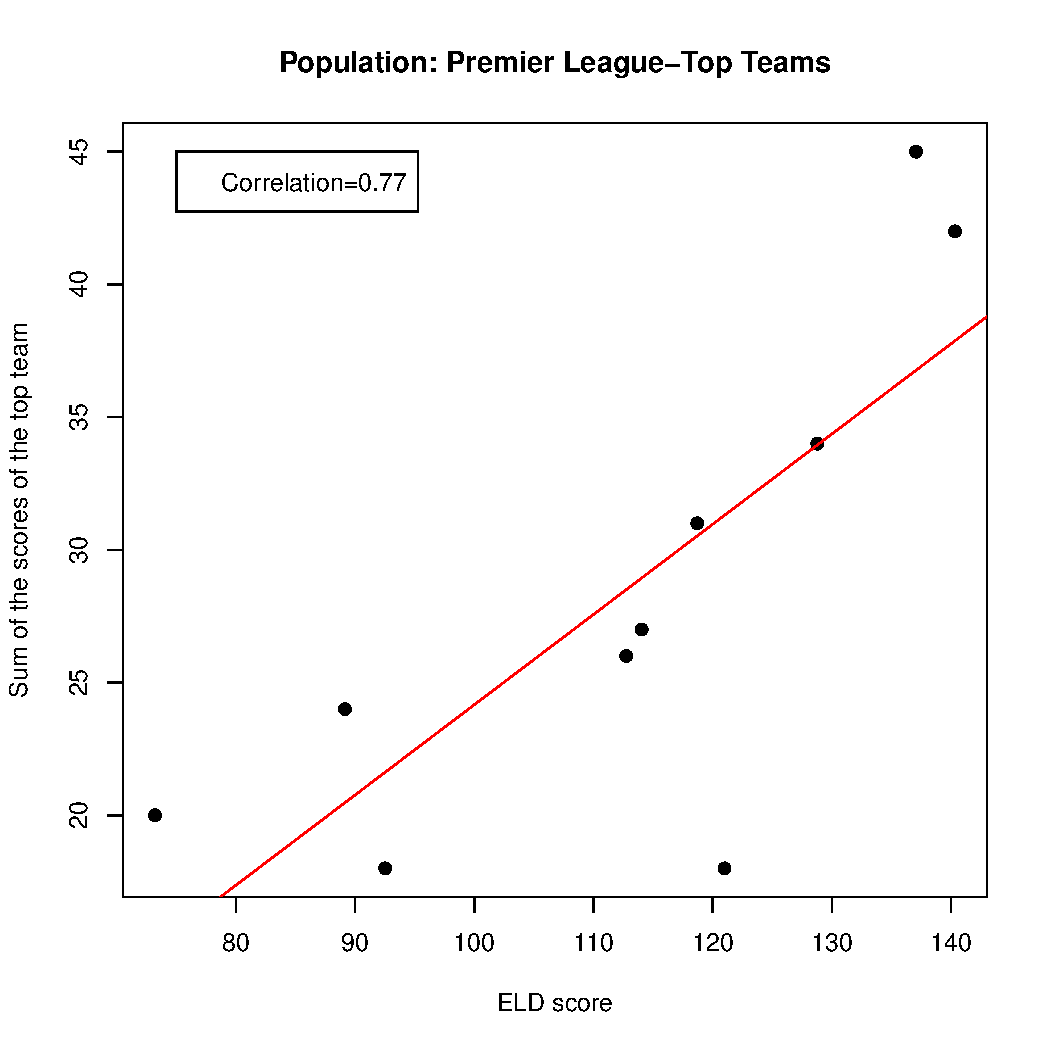
\includegraphics[width=0.5\textwidth]{NewPlotsJan2016/topTeamStats.pdf}}
			\caption{Correlations in the goalies population\label{fig:goaliesELD}}
		\end{figure}
		
		
		\paragraph{Midfielder Salary} 
		
		We omit a scatterplot for midfielder salary vs. $\mid$ because it is less informative due to the weaker  correlation (0.45).
		%
		%While there is a strong correlation between salary of the Strikers and ELD score (0.79), this correlation becomes weaker in the Goalie population and even less apparent in Midfielder group. 
		To investigate the reason for the weaker correlation, we chose two midfielders: 1) Stephane Sessegnon  who has been ranked second in the $\mid$ ranking but does not draw a large salary and 2) Steven Gerrard is a very well known player and ranked second in the Salary ranking, but according to the $\mid$ score, he has been ranked 21. Based on domain knowledge, we chose some of the features from the raw data that are relevant to midfield performance and compared the feature statistics for these two players. Table~\ref{table:MidfielderComparison} shows the details of their appearances in different matches. Sessegnon scored higher than Gerrard in three out of the four categories (Passes and Time Played). However, his salary was much lower than Gerrard's. This is an example of how weak the correlation is between salary and the observed box scores, which is the basis for the $\mid$ metric. 
		%to show how unfair and unreliable the salary is in this domain.
		%	 Unsuccessful Passes&Successful Long Passes
		\begin{table}[htbp]
			
			\centering
			\resizebox{1\textwidth}{!}{
				\begin{tabular}{|l|l|c|c|c|c|c|c|c|}
					\hline
					Name&Team&age&\begin{tabular}{c}Salary\\Ranking \end{tabular}&\begin{tabular}{c}$\mid$\\Ranking \end{tabular}&\begin{tabular}{c}Time\\Played \end{tabular}&\begin{tabular}{c}Unsuccessful\\Passes \end{tabular}&\begin{tabular}{c}Successful\\Long Passes \end{tabular}&\begin{tabular}{c}Successful\\corners \end{tabular}\\\hline
					Steven Gerrard	&Liverpool&31&2&21&1212 min&244&52&25\\\hline
					Stephane Sessegnon&Sunderland&26&22&2&3133 min&231&82&15\\\hline
					
					%	$\mid$&0.71&0.73&0.6\\\hline
				\end{tabular}}
				%
				\caption{Comparison of two midfielders.\label{table:MidfielderComparison}}
			\end{table}
			
			
			\subsubsection{Movies} 
			
			\paragraph{Movie Sum of Ratings} is the number of user ratings of a movie. Table~\ref{table:ELDmovie} shows a high correlation with the $\mid$ metric. The highest correlation obtained is for the Comedy genre (0.85). 
			%See Figure~\ref{fig:ActionRate},Figure~\ref{fig:ComedyRate}, Figure~\ref{fig:DramaRate}). 
			The correlation between a movie and the sum of its ratings is equally strong, but the correlation with its average rating is much weaker. Thus, the $\mid$ score is mainly related to how many users have rated the movie rather than with how they have rated it. The number of ratings is a meaningful success metric as it indicates the number of people who have gone to see a movie.  
			
			
			Figure~\ref{fig:Movies} shows the correlation of $\mid$ with movie success metrics in a scatter plot. We again observe a large cluster of movies around the origin. For drama and comedy movies, the top rated movies are (``American Beauty'' resp. ``Being John Malkovich''); these also stand out in the $\mid$ metric. 
			
			
			\begin{figure}
				\centering     %%% not \center
				\subfigure[Action movies: sum of ratings by users vs $\mid$. ]{\label{fig:ActionRate}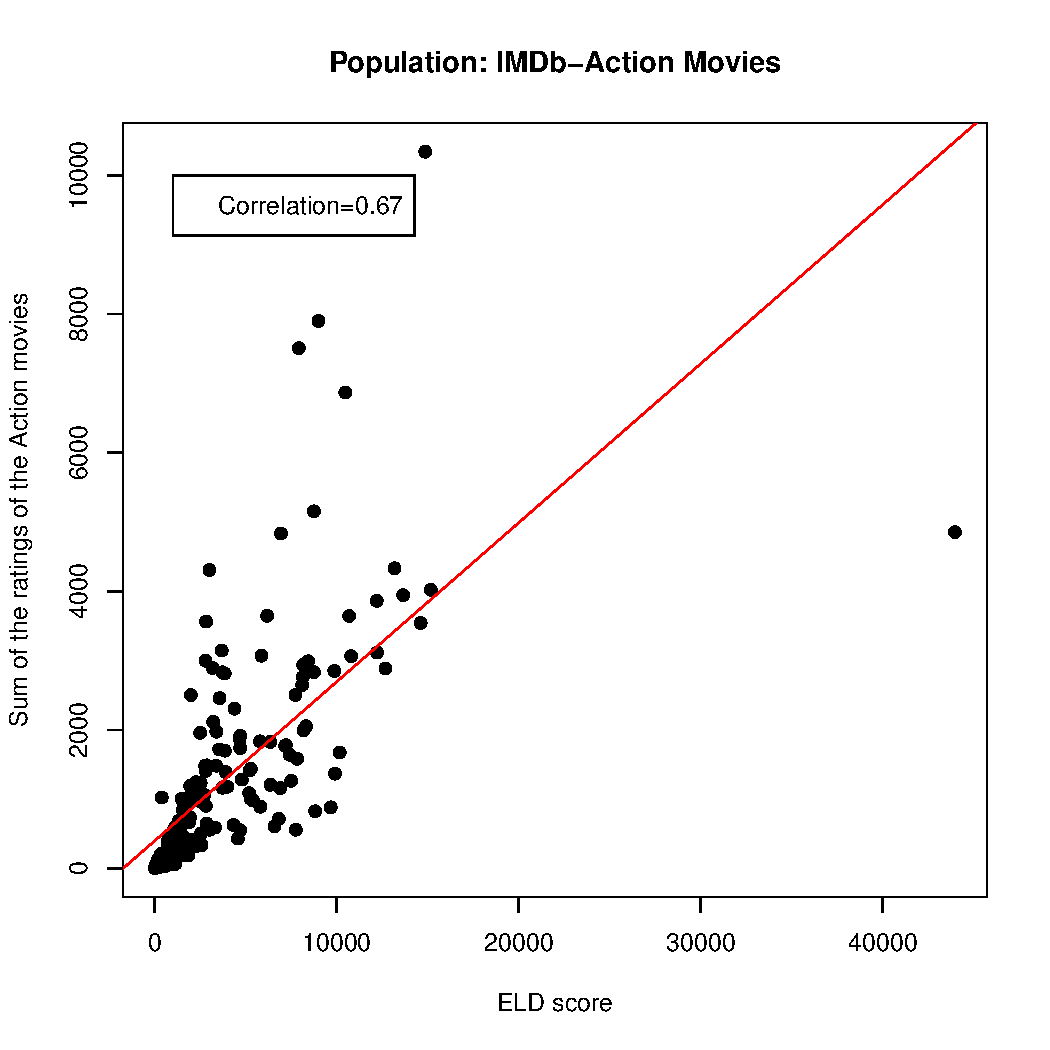
\includegraphics[width=0.48\textwidth]{NewPlotsJan2016/Action-Correlation.pdf}}
				\subfigure[Comedy movies: sum of ratings by users vs $\mid$]{\label{fig:ComedyRate}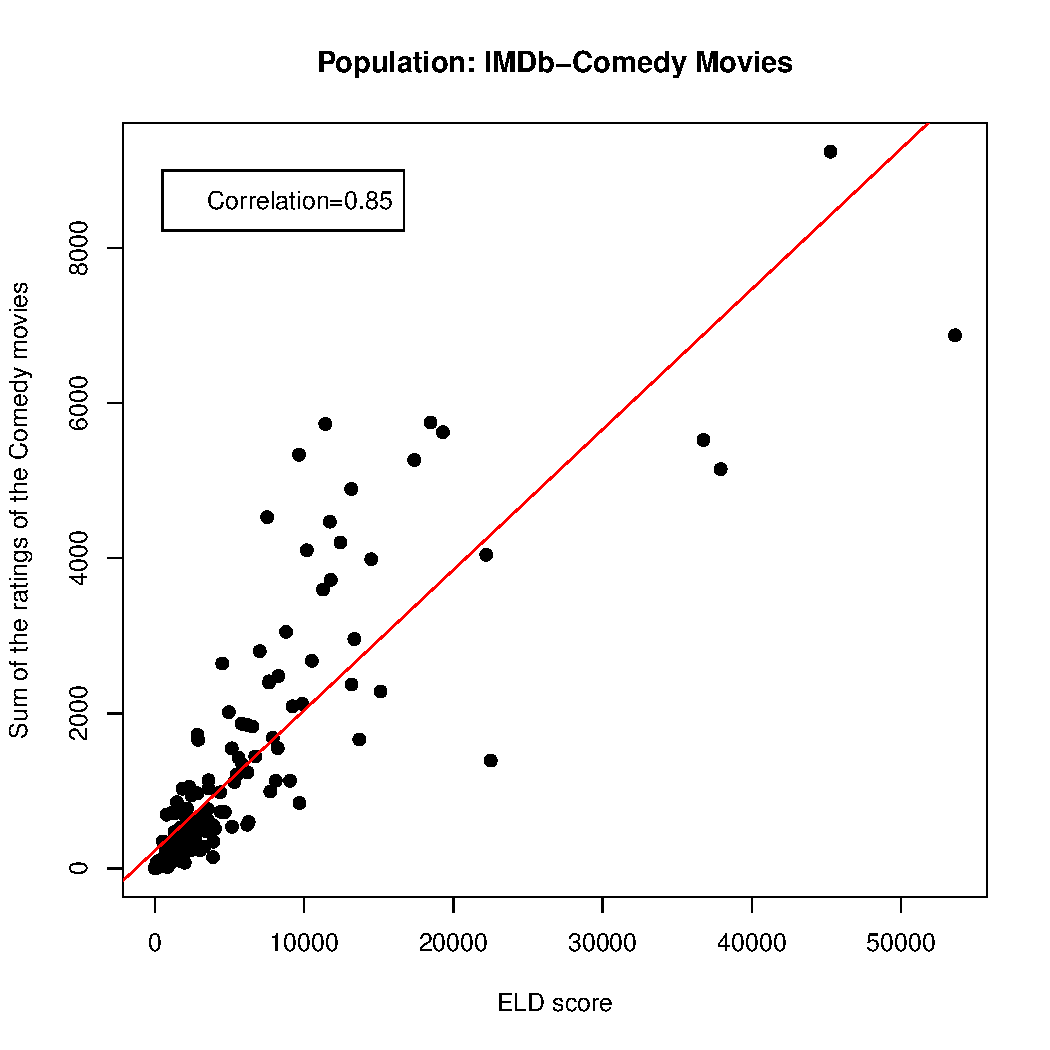
\includegraphics[width=0.5\textwidth]{NewPlotsJan2016/Comedy-Correlation.pdf}}
				\subfigure[Drama movies: sum of ratings by users vs $\mid$.]{\label{fig:DramaRate}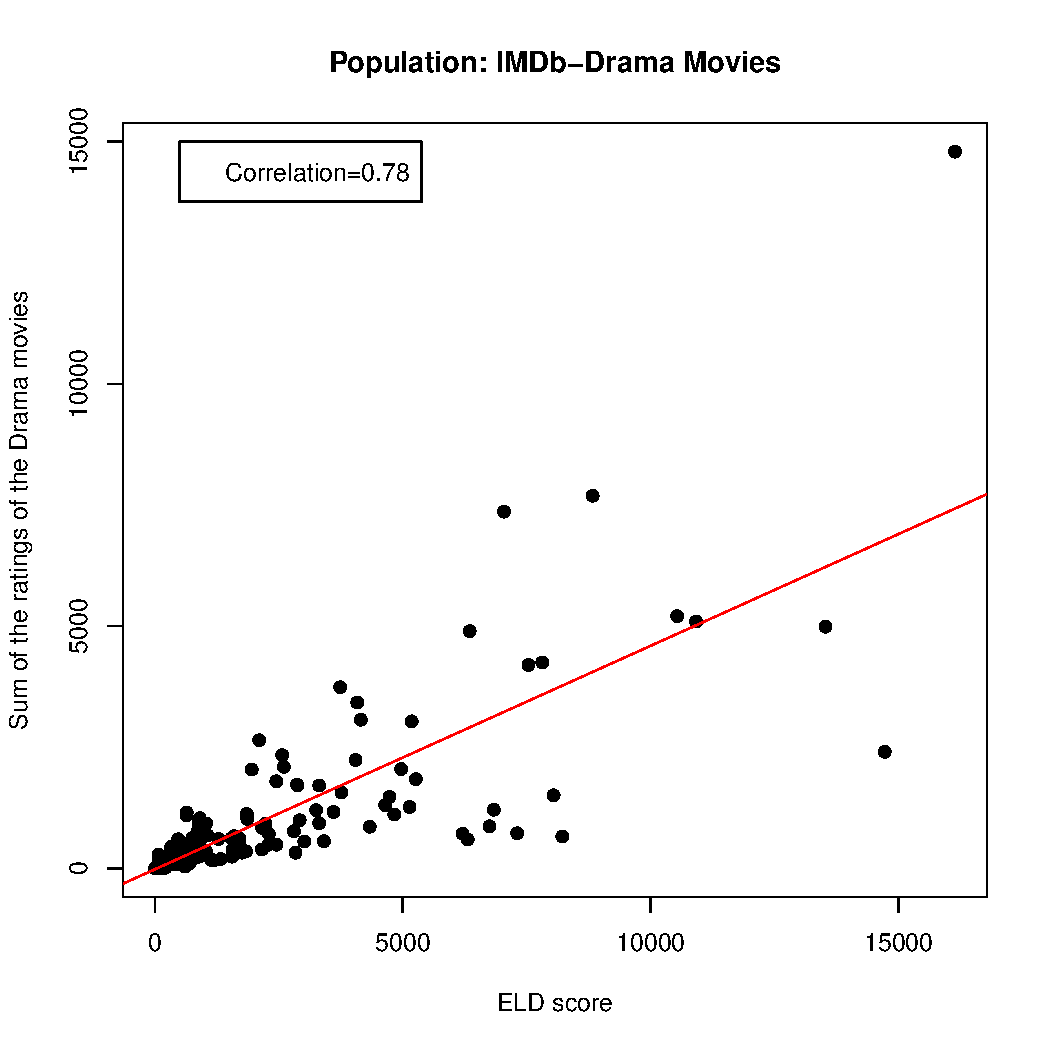
\includegraphics[width=0.5\textwidth]{NewPlotsJan2016/Drama-Correlation.pdf}}
				\caption{Correlation in the movies population\label{fig:Movies}}
			\end{figure}
			
			
\section{Conclusion}
In this chapter we used the $\mid$ metric, that was introduced in chapter~\ref{chap:five}, to rank the individuals. We compared the $\mid$ metric to other metrics of success for a given domain.
In our experimental results we showed that the $\mid$ metric correlates with success metrics, to a surprising degree, across different domains and classes of individuals. Since high success is an independent metric that indicates an unusual individuals, this correlation shows that $\mid$ marks meaningful and interesting outliers.

We investigated some independent factors that affect the success of individuals in the Premier League. We showed that there are factors other than the performance of players that affect their ranking and for this reason the methods that are solely based on evaluation of the performance of players can never achieve 100$\%$ accuracy in predicting the ranking. 


%\paragraph{Soccer Data} 
%The Opta data were released by Manchester City. 
%It lists all the ball actions within each game by each player, for the 2011-2012 season. 
%%The data consists of information about the actions of a single player in a given match 
%%from 2011 to 2012. 
%%Number of goals, passes, fouls, tackles, saves and blocks and also position 
%%assigned to a player in a match are examples of the information associated with each player. [list]
%%Information about the teams in a season, such as number of home wins, draws or away wins can be extracted by massaging the data. 
%%[The information can be visualized as a heterogeneous network that links players to teams, and teams to matches. ]
%For each player in a match, our data set contains eleven player features.
%% like $\it{TimePlayed}(\P,\M)$.
%For each team in a match, there are five features computed as player feature aggregates, as well as the team formation and the result (win, tie, loss). 
%There are two relationship terms, $\it{Appears\_Player}(\P,\M)$, $\it{Appears\_Team}(\T,\M)$. We store the data in a relational database, with a table for each base population and a table for each relationship.

%Six team f aggregates of player features. 
% like $\it{shoteff}(\team,\match)$. 
%The 11 player features are \\ 
%
%$\it{TimePlayed}$, $\it{SavesMade}$, $\it{ShotEff}$,
% $\it{FirstGoal}$, $\it{WinningGoal}$, $\it{Goals}$,$\it{PositionID}$, $\it{PassEff}$, $\it{TackleEff}$,$\it{DribbleEff}$,
% $\it{ShotsOnTarget}$\\
%
%\paragraph{IMDB Data} 
%
%The Internet Movie Database (IMDB) is an online database of information related to films, television programs, and video games.
%The IMDB website offers a dataset containing a information on cast, crew, titles, technical details and biographies into a set of compressed text files. 
%We preprocessed the data \cite{Peralta2007} to obtain a database with seven tables: one for each population and one for the three relationships $\it{Rated}(\user,\movie)$, $\it{Directs}(\director,\movie)$, and $\it{ActsIn}(\actor,\movie)$.

	
%\section{Likelihood Ratio and Success Metrics}
%The aim of this section is to compare the ELD metric with other meaningful success metrics for comparing individuals. Our reference metrics are success rankings of individuals, shown in table~\ref{table:successmetrics}. Strong correlations between the ELD metric and meaningful success metrics provide evidence that the ELD metric is meaningful as well. We measure correlation strength by the standard correlation coefficient $\rho$. The coefficient ranges from -1 to 1, where 0 means no correlation and 1 or -1 indicates maximum strength~\cite{Fisher1921}.\\
%
%Correlations are remarkable in at least two respects. 1) the strength of the correlation between the ELD metric and the success ranking are high: coefficients range from 0.3 to 0.82. (Oliver: correlation between ELD and movie rank is not as high as sum of ratings, should we just drop that or keep it? see table~\ref{table:movie}). 2) The trend holds across two different domains, different types of individuals and different success metrics. 
%\begin{table}[htbp]
%	
%	\centering
%	\resizebox{0.8\textwidth}{!}{
%		\begin{tabular}{|l|l|l|l|l|l|}
%			\hline
%			Dataset&Success Metric&Min&Max&Standard Dev.&Mean\\ \hline
%			IMDb & Sum of Rating & 1.8 & 9 & 1.14 & 6.3\\ \hline
%			Soccer-Player &TimePlayed& 5.0 & 3420 & 1015.69 & 1484.0\\ \hline
%			Soccer-Player&Normalized Salary&s&s&s&s\\\hline
%			Soccer-Player&Sum of Shot Efficiency&s&s&s&s\\\hline
%			Soccer-Team &Sum of Score& 1.0 & 20 & 5.91 & 10.5\\ \hline
%			
%		\end{tabular}}
%		\caption{Success metrics. \label{table:metrics}}
%		
%	\end{table}
%
%The quality of generalization of population is the key to the performance of ELD metric in ranking individuals. For example, in Premier League we expect most players to be in the range of good players. So the more different a player is from the population we can interpret it as a sign of detecting exceptionally good players. If we have a more diverse population in terms of performance, apart from a serious decline in quality of generation, being different from generic model can be interpreted as both exceptionally better or worst than normal population.\\
%Another point to consider is that, in BN generalization, similar to statistical generalization, population size and the structure of the  individuals is important. For example, in the Premier League, when the goal is to predict the success of  teams, there is no strong correlation between the ELD metric and standing of the teams as we expected it to be similar to the other domain/individuals ($\rho(Standing, ELD)=-0.21$). This could be due to the diverse and yet very small population (20 teams in total). But when we decrease diversity by considering only top 10 teams in our evaluation, correlation becomes a lot more stronger ($\rho(Standing, ELD)=-0.71$).
%\paragraph{Team Standing}
%The most successful team has Standing=1 and the least successful team has Standing=20. If we distinguish top teams in the standing, a strong negative correlation emerges between ELD and standing: teams with higher ELD achieve a better(lower) standing. Figure~\ref{fig:teamStanding} shows the scatter plot of this correlation and its best fit regression line.
%\paragraph{Players Time Played} is the total time that a player played over all matches in the season. This metric was shown to correlate strongly with other success metrics, such as salary, on MLS soccer data~\cite{schwartz}. Tables ~\ref{table:goalie} and \ref{table:strikers} and Figures \ref{fig:GoalieTime} and \ref{fig:StrikerTime} show the correlation between the ELD metric and time played. For the the entire population there is a strong positive correlation meaning that atypical players with higher ELD tend to play more minutes.
%\paragraph{Salary} is probably the most obvious way of comparing players. We manually collected salary of some Strikers that we could find on-line. Table \ref{table:strikers}  and Figures~\ref{fig:NormalizedSalary} show the correlation between ELD and this success metric.
%\paragraph{Shots on Target} is any shot attempt that would or does enter the goal if left unblocked. We record total number these shots over all matches of the players. This metric was shown to correlate strongly with ELD (see Table \ref{table:strikers}, Figure~\ref{fig:StrikerShot}).
%\paragraph{Saves Made} is total number of saves that goalies had made over all the matches. This metric has been used as another success metric for Goalies' population and shows a strong correlation as well(see Table ~\ref{table:goalie}, Figure\ref{fig:GoalieSaves}).  
%\paragraph{Movie Rating} is the sum of user rating of the movies. For the movies in different Genre this metric shows a high correlation with the ELD metric (see Table~\ref{table:movie}, Figure~\ref{fig:ActionRate},Figure~\ref{fig:ComedyRate}, Figure~\ref{fig:DramaRate}).
%\begin{table}[htbp]
%	
%	\centering
%	\resizebox{0.7\textwidth}{!}{
%		\begin{tabular}{|c|c|c|}
%			\hline
%		Metric&Sum of SavesMade&TimePlayed\\\hline
%		ELD&0.71&0.73\\\hline
%		\end{tabular}}
%		%
%		\caption{Correlation between ELD metric and success metric of Goalies .\label{table:goalie}}
%	\end{table}
%	
%	\begin{table}[htbp]
%		
%		\centering
%		\resizebox{0.7\textwidth}{!}{
%			\begin{tabular}{|c|c|c|c|}
%				\hline
%				Metric&Shots On Target&TimePlayed& Salary\\\hline
%				ELD&0.72&0.82&0.79\\\hline
%			\end{tabular}}
%			%
%			\caption{Correlation between ELD metric and success metric of Strikers .\label{table:strikers}}
%		\end{table}
%		
%			
%			\begin{table}[htbp]
%				
%				\centering
%				\resizebox{0.5\textwidth}{!}{
%					\begin{tabular}{|c|c|c|}
%						\hline
%						Genre&Sum of Rating&Movie Rank\\\hline
%						Action&0.68&0.30\\\hline
%						Drama&0.78&0.31\\\hline
%						Comedy&0.85&0.42\\\hline
%				\end{tabular}}
%					%
%					\caption{Correlation between ELD metric and success metric of Movies .\label{table:movie}}
%				\end{table}
%				
%%	\begin{figure}[t]
%%		\centering
%%		\includegraphics[width=0.8\textwidth] 
%%		{correlations/Drama-Correlation.pdf}
%%		\caption{
%%			Salaries of players across different nationalities. 
%%			\label{fig:nationalitySalary}
%%		}
%%	\end{figure}			
%%\begin{figure}
%\begin{figure}
%	\centering
%	\begin{minipage}{0.45\linewidth}
%		\centering
%		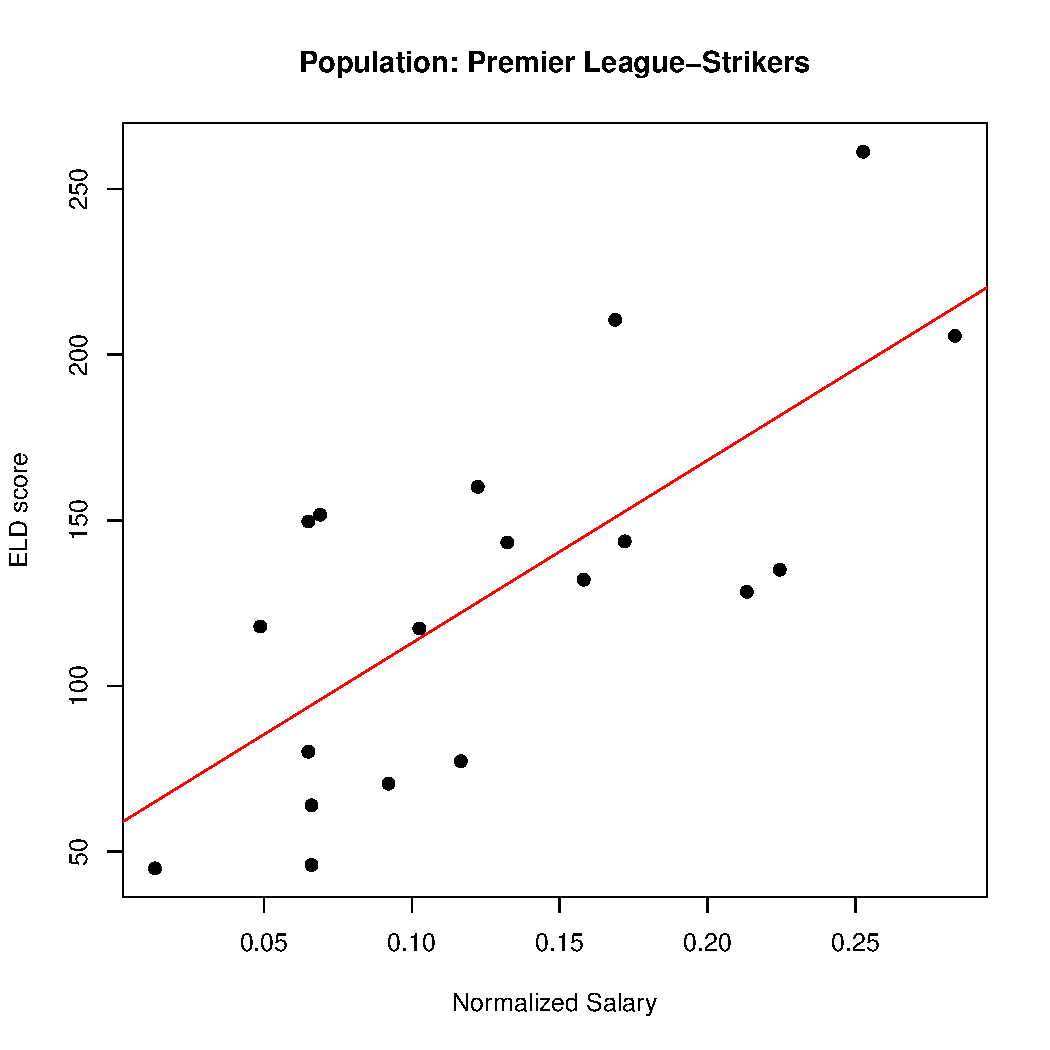
\includegraphics[width=3.0in]{Correlation-SimplePlots/1d-sumStrikerSalary.pdf}
%		\caption{Strikers: Salary vs ELD}
%		\label{fig:StrikerSalary}
%	\end{minipage}
%	\hspace{0.05\linewidth}
%		\begin{minipage}{0.45\linewidth}
%			\centering
%			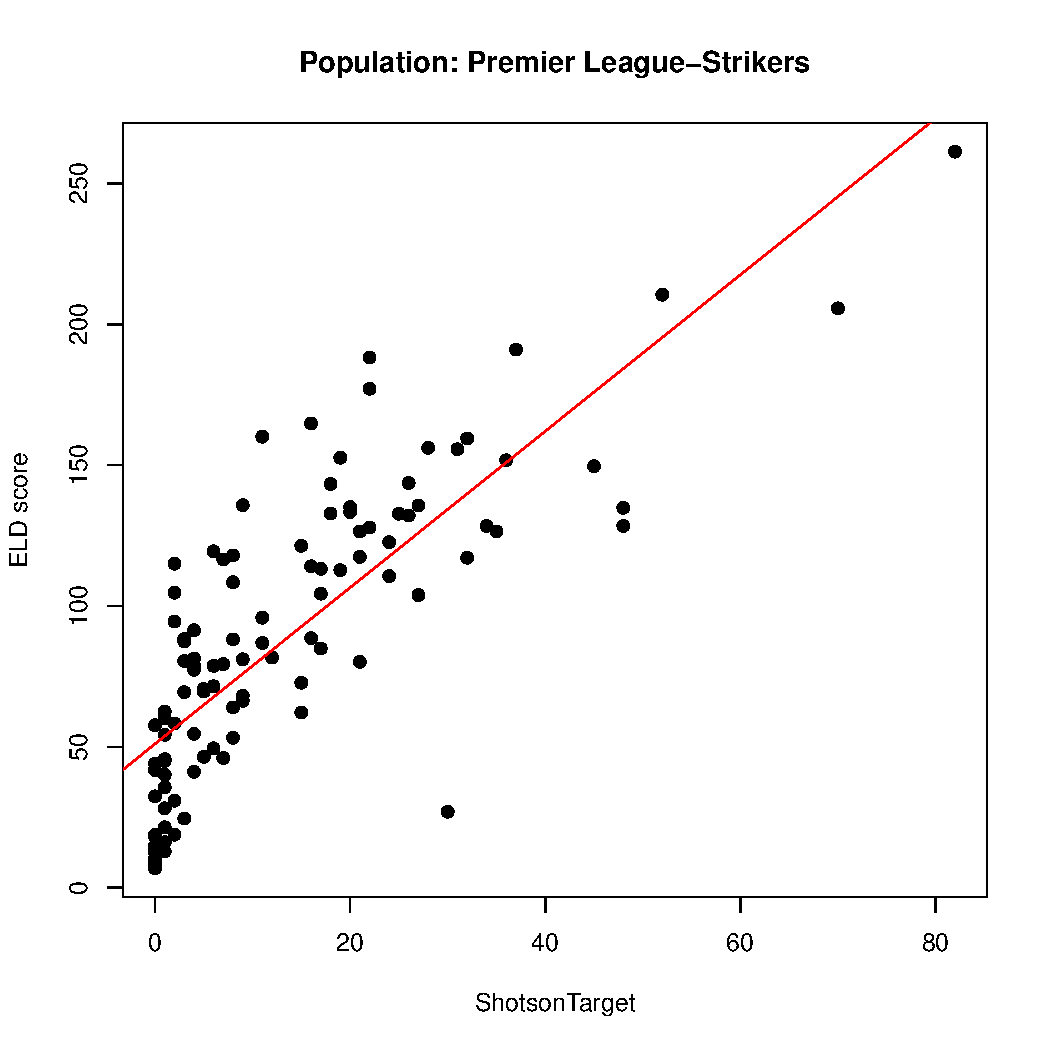
\includegraphics[width=3.0in]{Correlation-SimplePlots/1d-ShotsonTarget-sumStrikerStatistics.pdf}
%			\caption{Strikers: Shots On Target vs ELD}
%			\label{fig:StrikerShot}
%		\end{minipage}
%			\hspace{0.05\linewidth}
%			\begin{minipage}{0.45\linewidth}
%				\centering
%				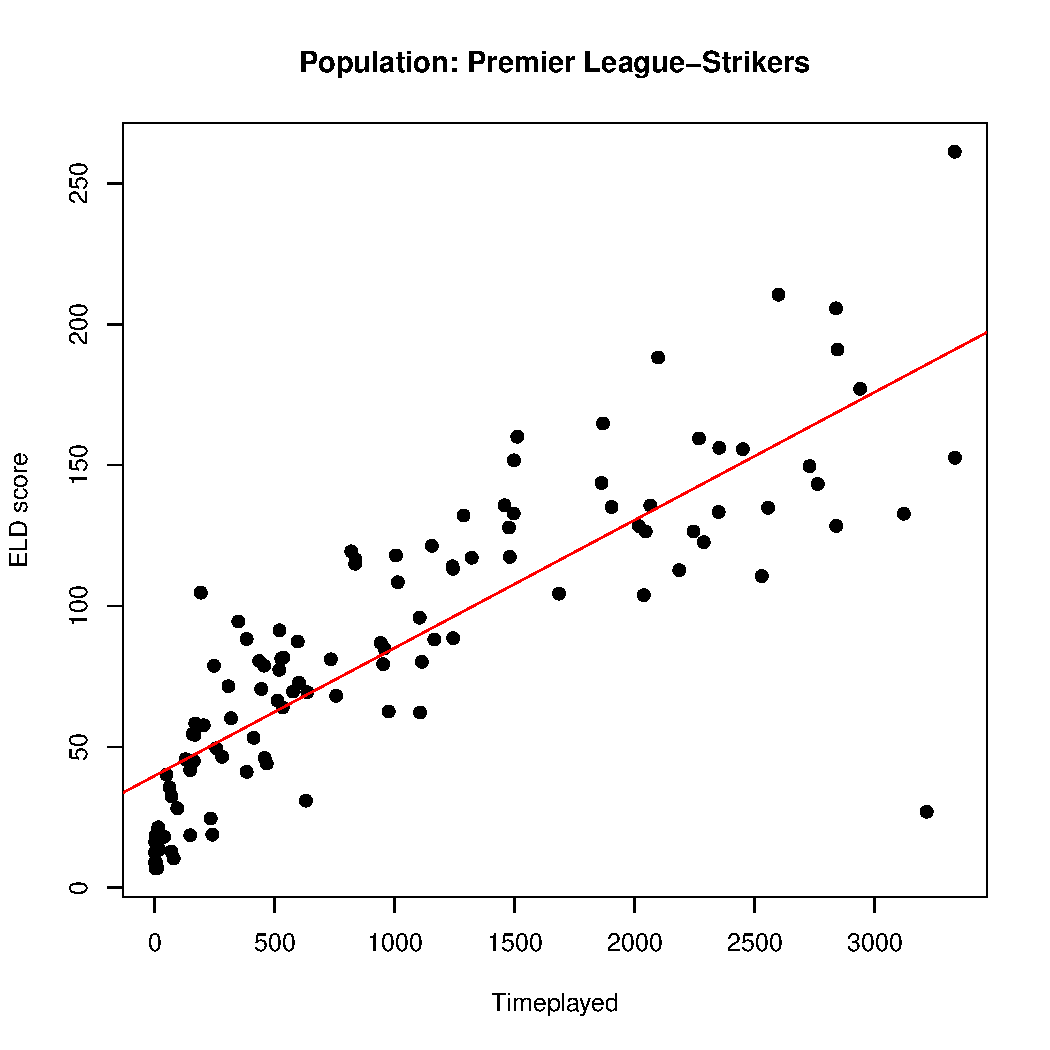
\includegraphics[width=3.0in]{Correlation-SimplePlots/1d-sumStrikerStatistics.pdf}
%				\caption{Strikers: Time played vs ELD}
%				\label{fig:StrikerTime}
%			\end{minipage}
%\end{figure}
%
%\begin{figure}
%	\centering
%	\begin{minipage}{0.45\linewidth}
%		\centering
%		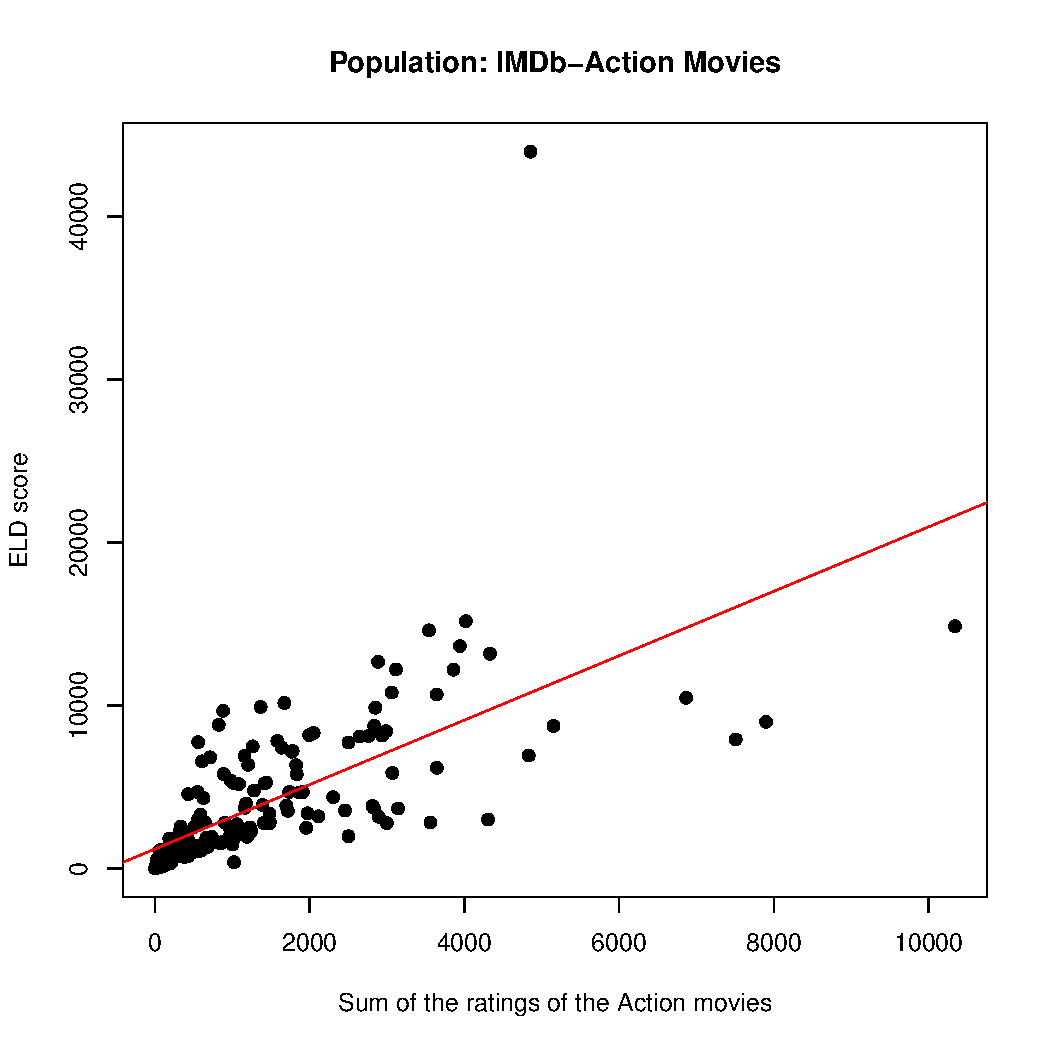
\includegraphics[width=3.0in]{Correlation-SimplePlots/Action-Correlation.pdf}
%		\caption{Action movies: sum of ratings by users vs ELD}
%		\label{fig:ActionRate}
%	\end{minipage}
%	\hspace{0.05\linewidth}
%	\begin{minipage}{0.45\linewidth}
%		\centering
%		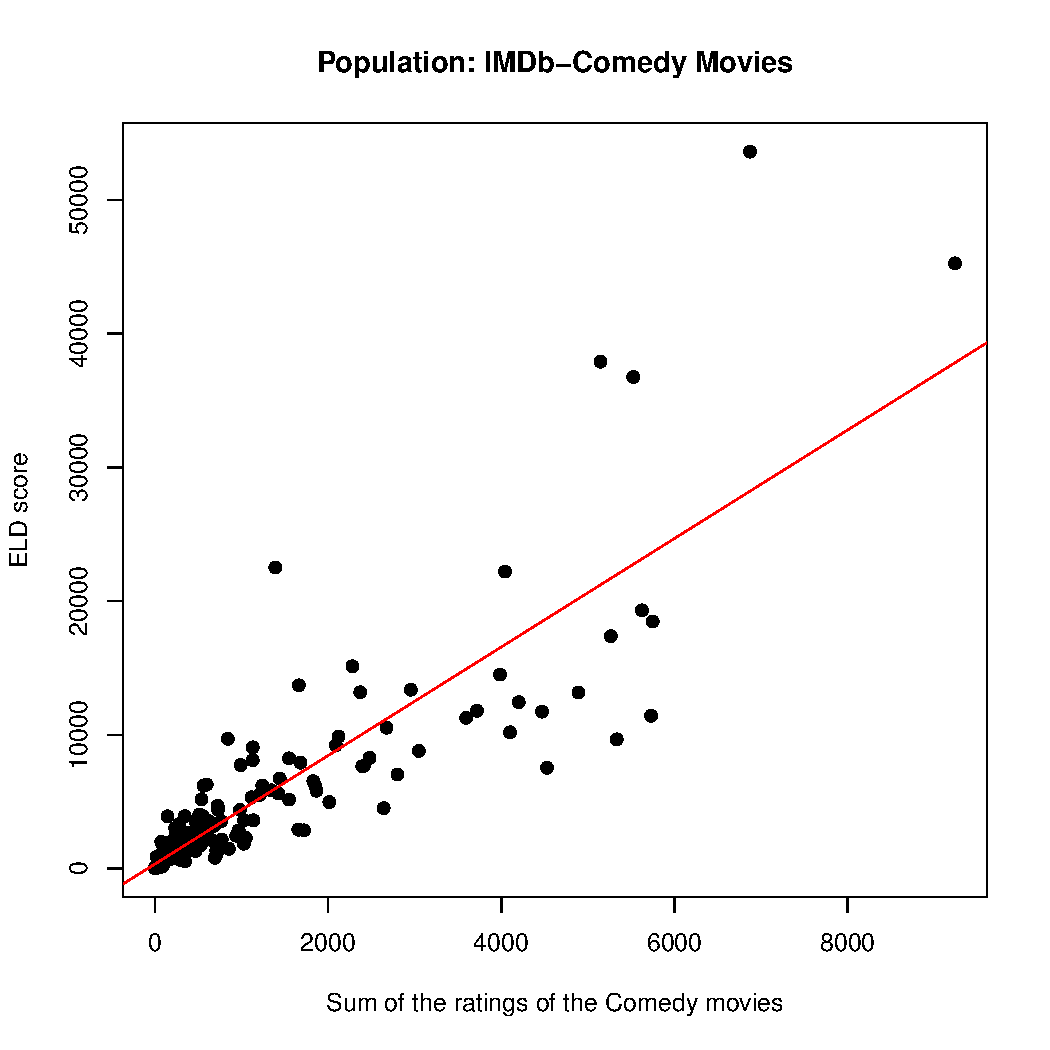
\includegraphics[width=3.0in]{Correlation-SimplePlots/Comedy-Correlation.pdf}
%		\caption{Comedy movies: sum of ratings by users vs ELD}
%		\label{fig:ComedyRate}
%	\end{minipage}
%	\hspace{0.05\linewidth}
%	\begin{minipage}{0.45\linewidth}
%		\centering
%		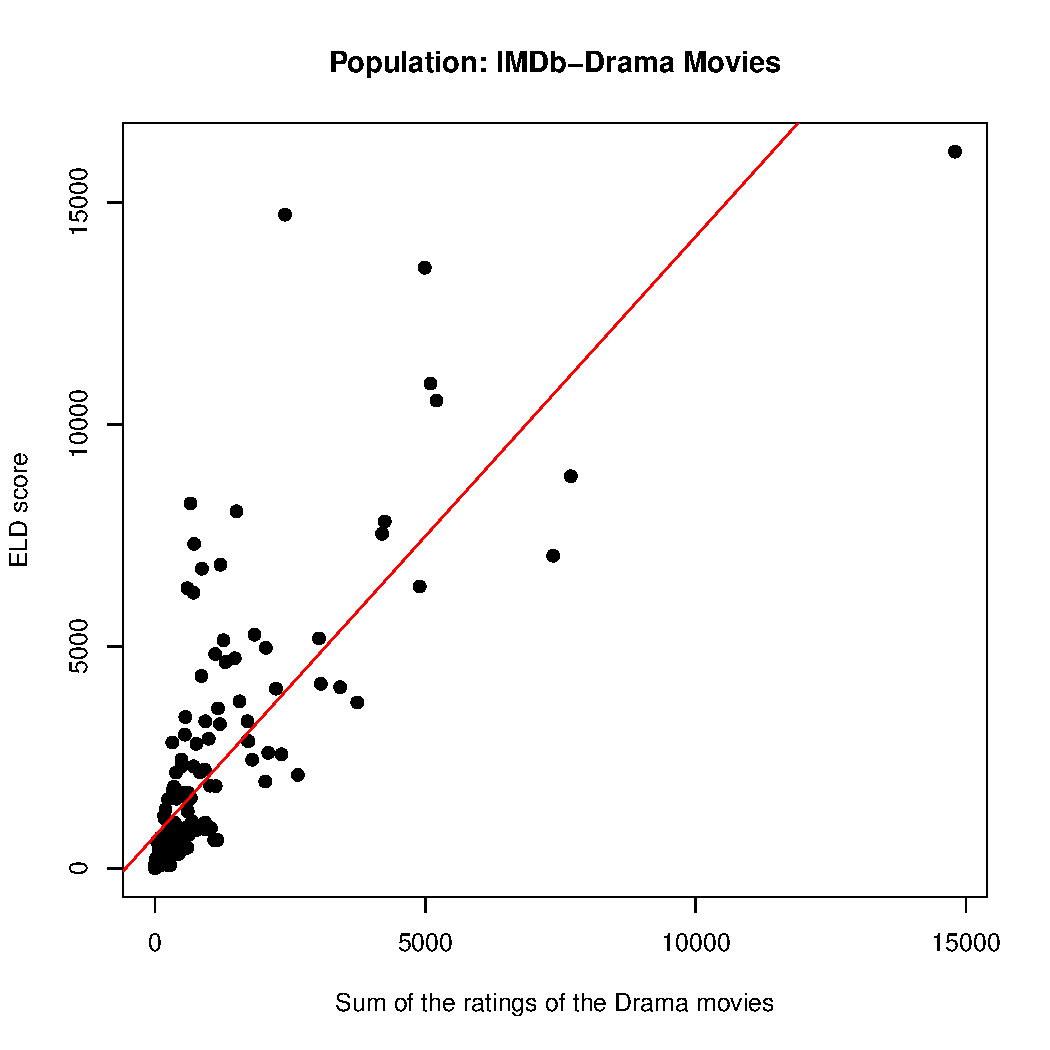
\includegraphics[width=3.0in]{Correlation-SimplePlots/Drama-Correlation.pdf}
%		\caption{Drama movies: sum of ratings by users vs ELD}
%		\label{fig:DramaRate}
%	\end{minipage}
%\end{figure}
%
%				
%				
%				
%				\begin{figure}
%					\centering
%					\begin{minipage}{0.45\linewidth}
%						\centering
%						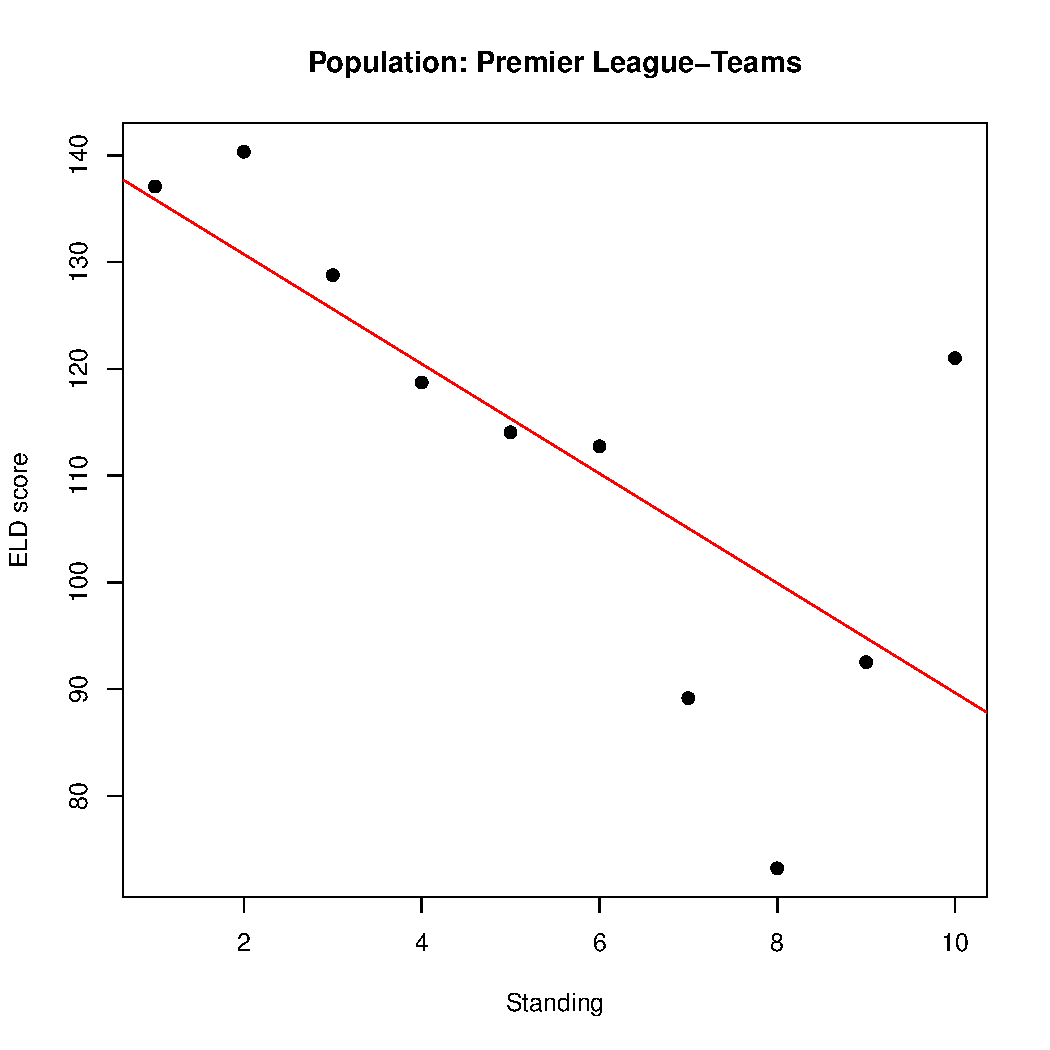
\includegraphics[width=3.0in]{Correlation-SimplePlots/TeamStanding.pdf}
%						\caption{Teams: Correlation between team's Standing and ELD for the top teams in Premier League standing}
%						\label{fig:teamStanding}
%					\end{minipage}
%					\hspace{0.05\linewidth}
%					\begin{minipage}{0.45\linewidth}
%						\centering
%						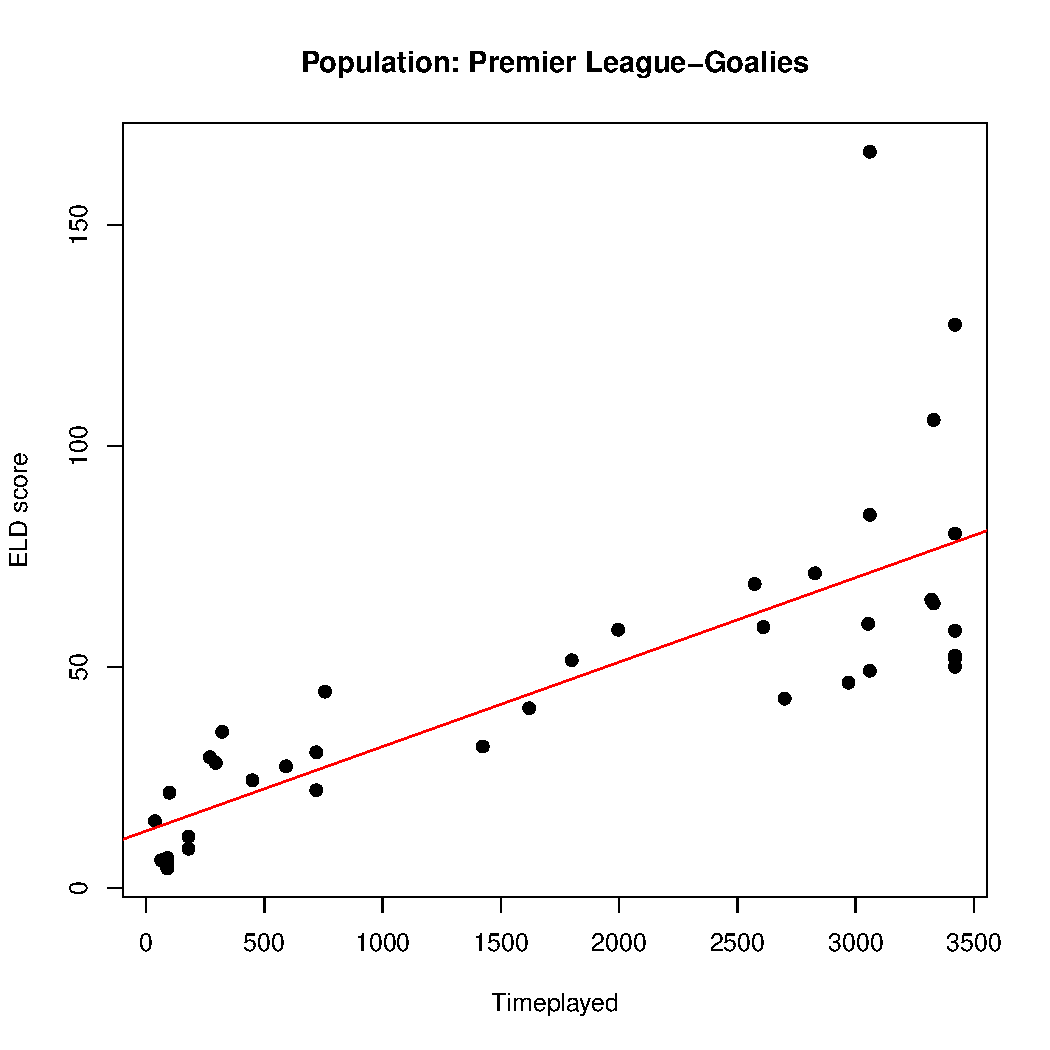
\includegraphics[width=3.0in]{Correlation-SimplePlots/sumGoalieStatistics.pdf}
%						\caption{Goalies: sum of time played vs ELD}
%						\label{fig:GoalieTime}
%					\end{minipage}
%					\hspace{0.05\linewidth}
%					\begin{minipage}{0.45\linewidth}
%						\centering
%						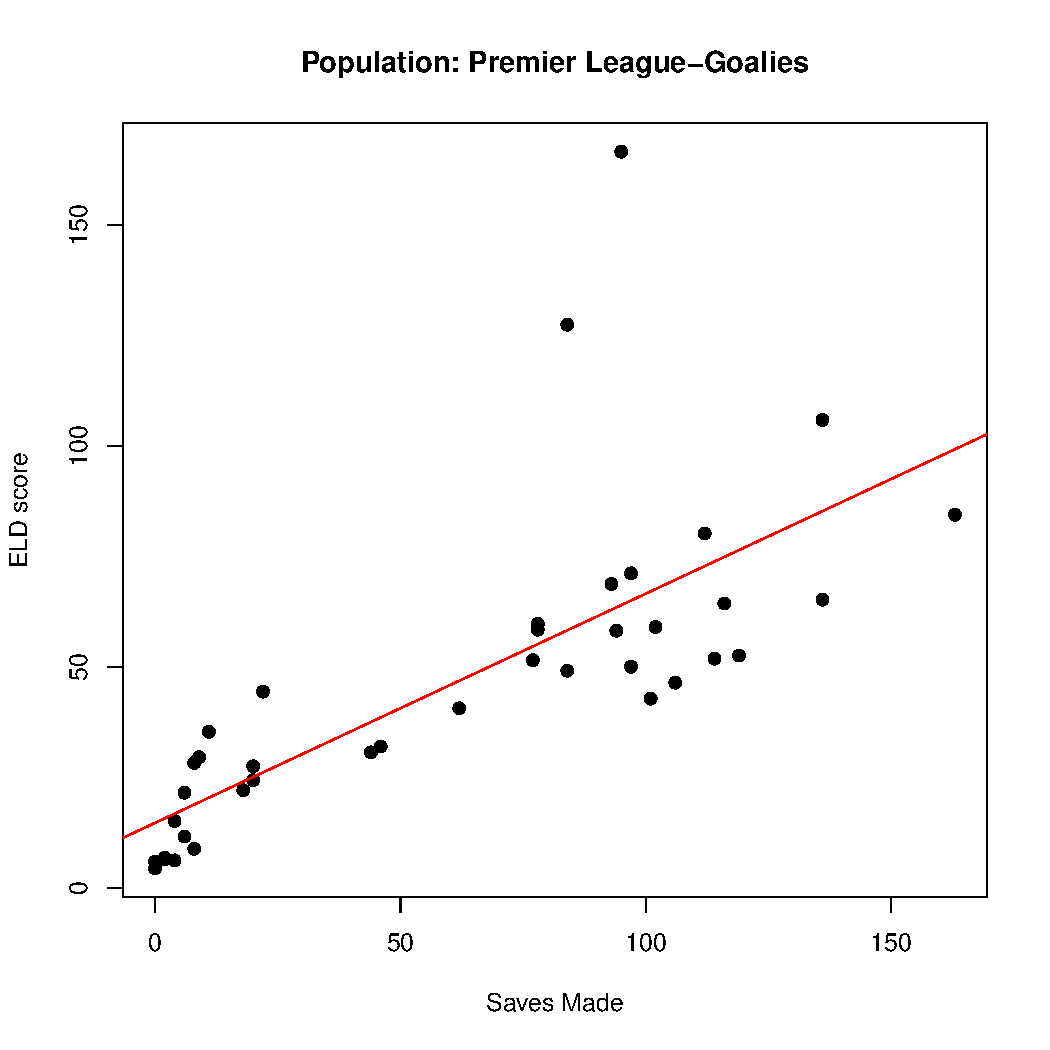
\includegraphics[width=3.0in]{Correlation-SimplePlots/sumGoalieStatisticsSavesMade.pdf}
%						\caption{Goalies: sum of saves made by users vs ELD}
%						\label{fig:GoalieSaves}
%					\end{minipage}
%				\end{figure}
%				
				
				
%					\begin{figure}[t]
%						\centering
%						\includegraphics[width=0.45\textwidth] 
%						{Correlation-SimplePlots/topTeamStats.pdf}
%						\caption{
%							Teams: Correlation between team's performance and ELD. 
%							\label{fig:nationalitySalary}
%						}
%					\end{figure}

%	\centering     %%% not \center
%	\subfigure[Figure A]{\label{fig:a}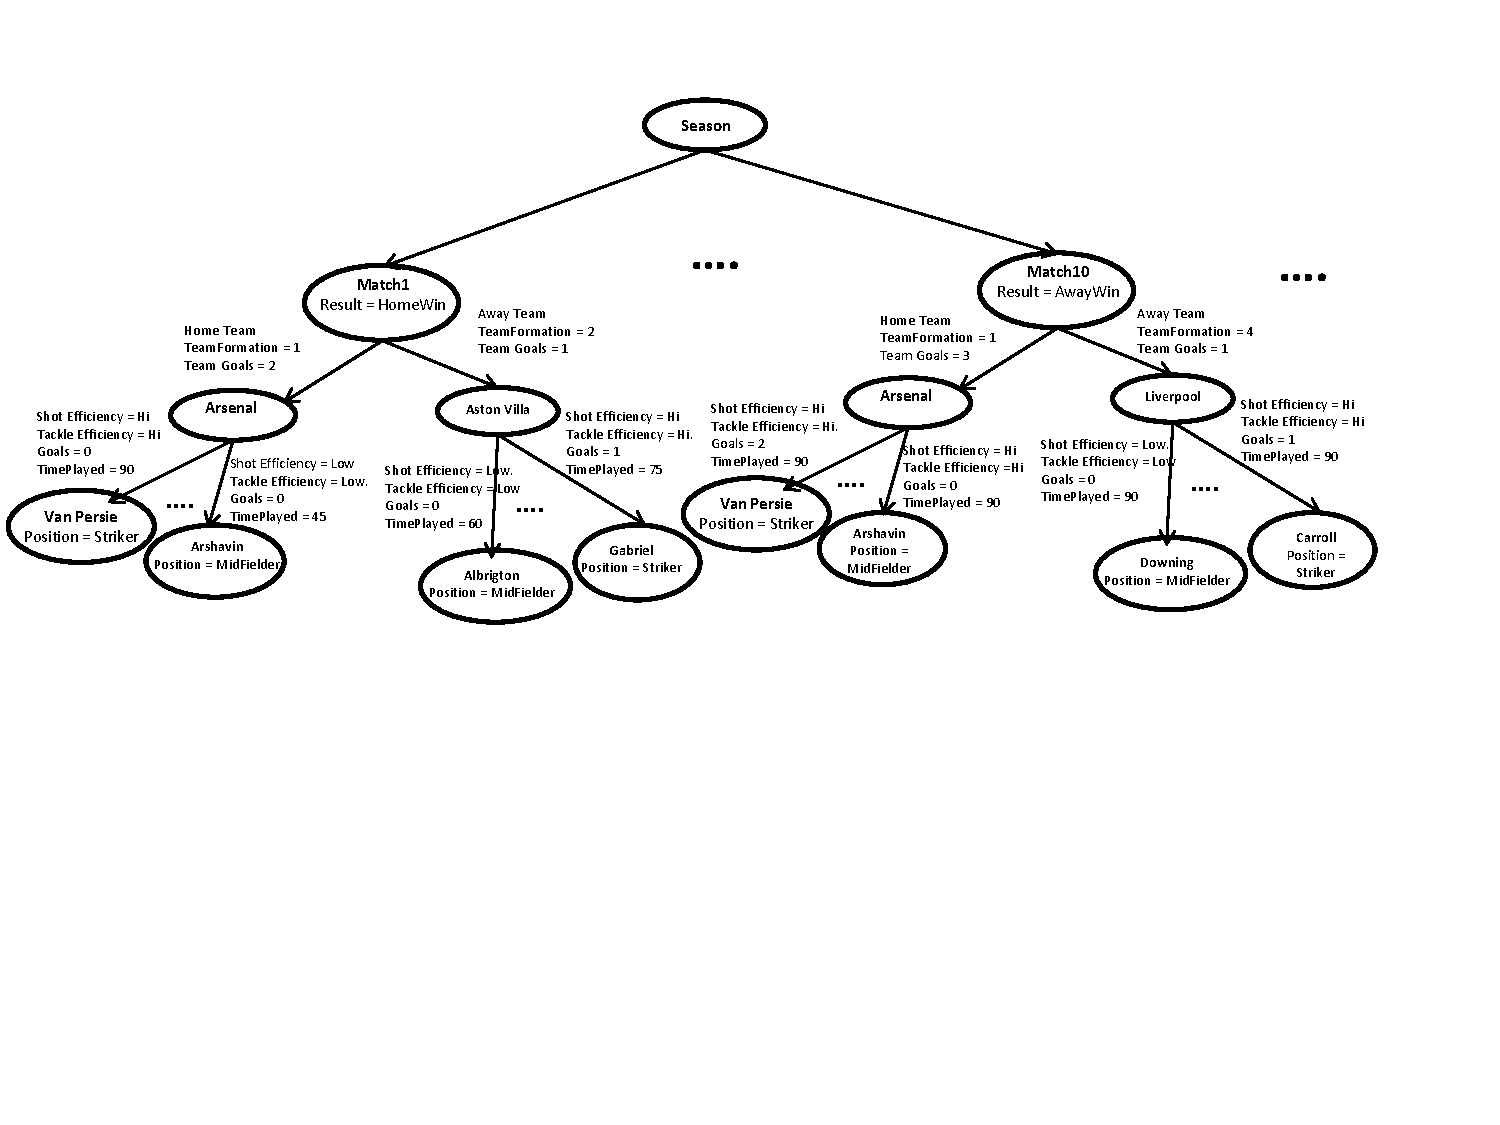
\includegraphics[width=60mm]{figures/SeasonGraph.pdf}}
%	\subfigure[Figure B]{\label{fig:b}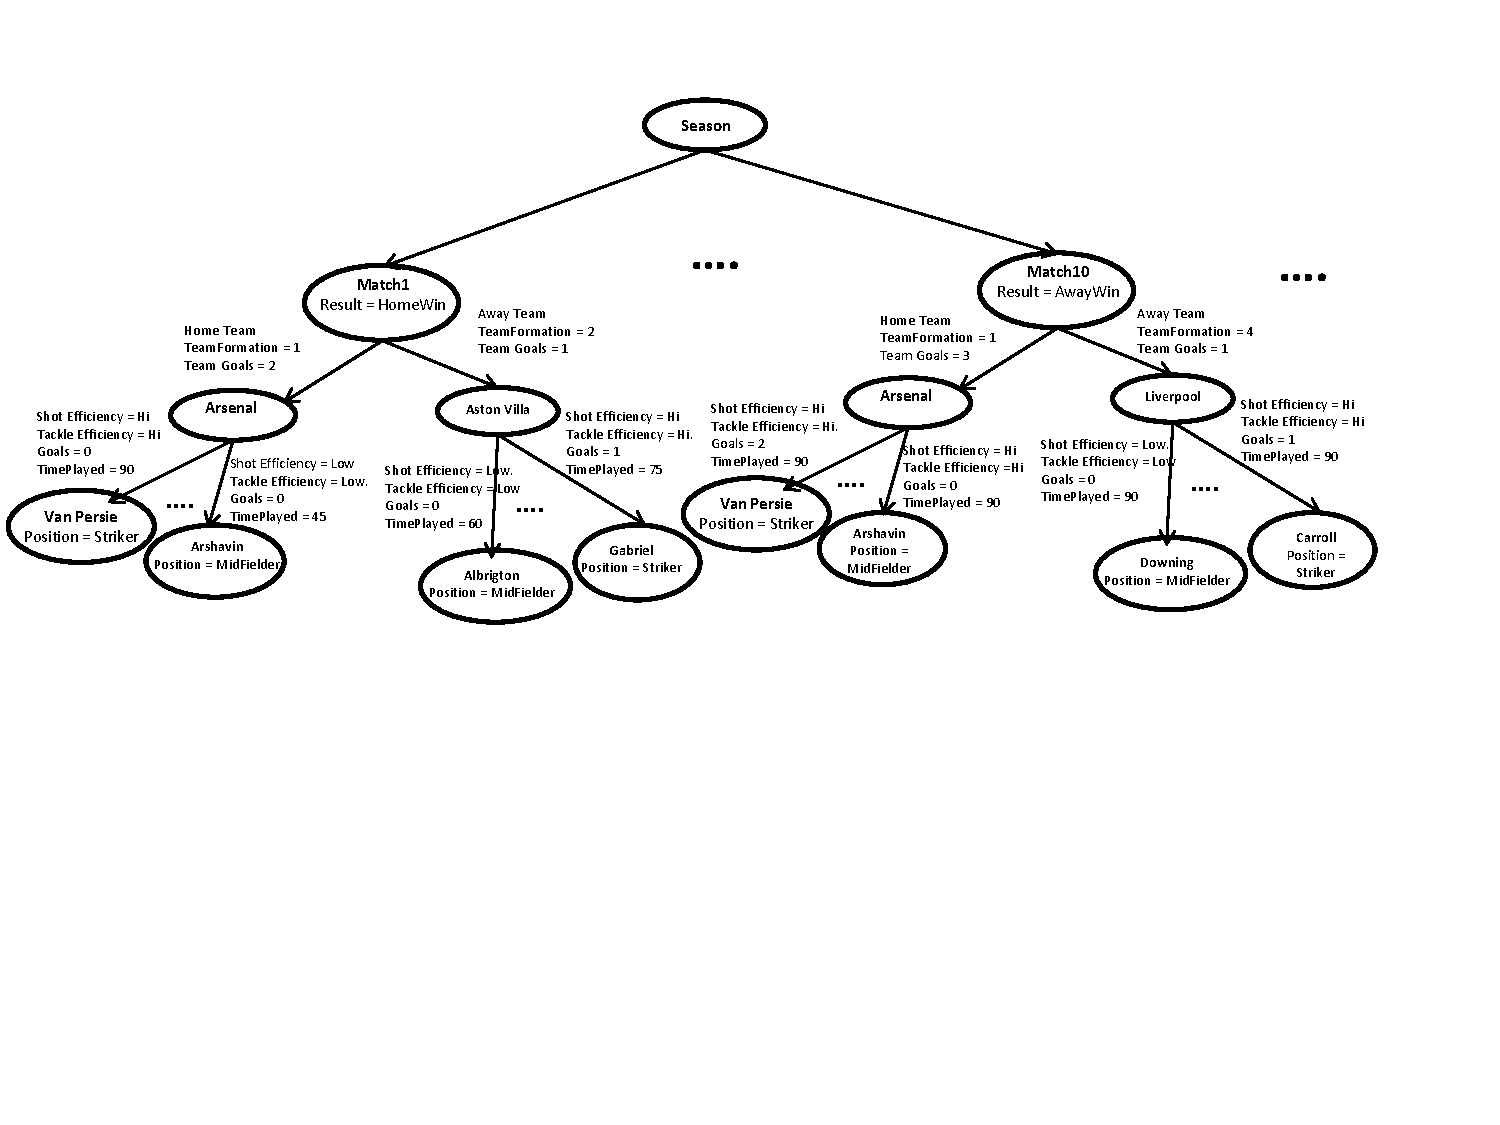
\includegraphics[width=60mm]{figures/SeasonGraph.pdf}}
%	\caption{my caption}
%\end{figure}
